\documentclass[11pt]{article}
% -----------------------------------------------------------------------------
% Response to the reviewers of MS CPENG-8674 (major revision, October 2026).
% Draft: answers are written only for the comments addressed so far.
% Code: MODULES/review29oct_fixed | Data: Data/03Nov_FINAL_GirderBearings_7D_5sensors_5modes | Figures: ./figures_final
% Orange text = notes for the authors and placeholders (remove or fill before submission).
% -----------------------------------------------------------------------------
\usepackage[a4paper,margin=2.5cm]{geometry}
\usepackage{amsmath,amssymb,bm}
\usepackage{graphicx}
\usepackage{booktabs,multirow,array,longtable,tabularx}
\usepackage{xcolor}
\usepackage{caption,subcaption}
\usepackage{float}
\usepackage{enumitem}
\usepackage{titlesec}
\usepackage{tikz}
\usetikzlibrary{decorations.pathmorphing,arrows.meta,calc,positioning,patterns,decorations.pathreplacing}
\usepackage[colorlinks=true,linkcolor=blue!50!black,citecolor=blue!50!black,urlcolor=magenta]{hyperref}

\definecolor{resp}{RGB}{25,70,170}
\definecolor{note}{RGB}{205,95,0}
\linespread{1.15}
\setlength{\parindent}{0pt}
\setlength{\parskip}{4pt}
\captionsetup{font=small,labelfont=bf,labelsep=colon}
\renewcommand{\thetable}{R\arabic{table}}
\renewcommand{\thefigure}{R\arabic{figure}}
\renewcommand{\theequation}{R\arabic{equation}}
\titleformat{\section}{\normalfont\large\bfseries}{}{0pt}{}
\titleformat{\subsection}{\normalfont\bfseries}{}{0pt}{}
\setlist{itemsep=1pt,topsep=2pt}

% --- Comment / response / action blocks (as in our previous response letters) ---
\newenvironment{rcomment}[1]{\par\bigskip\noindent\textbf{Comment\ifx&#1&\else\ #1\fi:}\ \itshape}{\par}
\newenvironment{response}{\par\smallskip\noindent\color{resp}\textbf{Response:}\ }{\par}
\newenvironment{action}{\par\smallskip\noindent\color{resp}\textbf{Action:}\ }{\par}
\newcommand{\pending}{\par\smallskip\noindent\textcolor{gray}{\textbf{Response:} \textit{pending --- this comment
has not been addressed yet.}}\par}
\newcommand{\authornote}[1]{\textcolor{note}{\textsf{[Authors: #1]}}}
\newcommand{\tbd}[1]{\textcolor{note}{\textsf{[#1]}}}
\newcommand{\lines}[1]{\tbd{lines #1}}

\newcommand{\m}{\mathbf{m}}
\newcommand{\z}{\mathbf{z}}
\newcommand{\f}{\mathbf{f}}

\begin{document}

\begin{center}
{\Large\bfseries Response to reviewer comments}\\[8pt]
\textbf{MANUSCRIPT ID:} CPENG-8674\\
\textbf{Date:} \today\\
\textbf{Title:} Uncertainty-aware damage identification in short-span bridges via physics-informed variational
autoencoder\\
\textbf{Journal:} Journal of Computing in Civil Engineering
\end{center}

\noindent\fcolorbox{note}{note!6}{\parbox{\dimexpr\linewidth-2\fboxsep-2\fboxrule}{\small\color{note}\textsf{%
\textbf{Draft status (\today).} Answers are given only for the comments addressed so far; the other comments are
reproduced with the mark ``pending''. Orange text is for the authors: notes, and placeholders for the results of the
training on the final dataset and for the line numbers of the revised manuscript. All numbers in blue come from the
final dataset (\texttt{Data/03Nov\_FINAL\_GirderBearings\_7D\_5sensors\_5modes}: girder line of a short-span composite
bridge on elastomeric bearings, five sensors, five modes) and the scripts in \texttt{MODULES/review29oct\_fixed}.}}}

\bigskip
We thank the Editor and the three reviewers for their careful reading of the manuscript and for their insightful and
constructive comments. They led us to rebuild the numerical case study, including the training, validation and test
datasets, and to revise the loss function so that the approximate posterior targets the Bayesian posterior. In the
following, we answer each comment point by point. Table~\ref{tab:summary} summarizes the responses and indicates where
the corresponding changes appear in the revised manuscript. Reviewer comments are reproduced in italics, and our
responses and the resulting actions are written in blue.

% =============================================================================
\section{Summary of the responses}
% =============================================================================
{\small
\begin{longtable}{p{1.55cm}p{6.0cm}p{3.0cm}p{3.6cm}}
\caption{Point-by-point summary of the responses.}\label{tab:summary}\\
\toprule
Comment & Topic & Status & Revised manuscript \\
\midrule
\endfirsthead
\toprule
Comment & Topic & Status & Revised manuscript \\
\midrule
\endhead
Editor & Validation, modelling uncertainty, boundary conditions, localized damage, $\gamma$, coverage & Partly addressed & See R1.1--R3.8 \\
R1.1 & Test data from a finer FE mesh & Addressed (VAE results pending) & \lines{xx--yy} \\
R1.2 & Model uncertainty and environmental variability & Addressed & \lines{xx--yy} \\
R1.3 & Coverage values (77.2\% vs.\ 0.789) and calibration & Addressed (results pending) & \lines{xx--yy} \\
R1.4 & Comparison with Refs.\ 39 and 41 & Addressed (results pending) & \lines{xx--yy} \\
R1.5 & Out-of-distribution test cases & Addressed (results pending) & \lines{xx--yy} \\
R1.6 & Localized, mild and healthy cases; false positives & Addressed (results pending) & \lines{xx--yy} \\
R1.7 & Finer discretization and scalability & Partly addressed & \lines{xx--yy} \\
R1.8 & Reference list & Pending (issues identified) & \\
R2.1 & Utility for real bridges in the introduction & Pending & \\
R2.2 & Realistic structure and elastic bearings & Addressed & \lines{xx--yy} \\
R2.3 & Damage parametrization, support conditions and detectable bearing damage & Addressed (VAE results pending) & \lines{xx--yy} \\
R2.4 & More realistic case study; laboratory beam & Partly addressed (no laboratory data) & \lines{xx--yy} \\
R3.1 & Robustness to modelling error (mass perturbation) & Addressed (results pending) & \lines{xx--yy} \\
R3.2 & Selection of $\gamma$ on the test set & Addressed (sensitivity study pending) & \lines{xx--yy} \\
R3.3 & Prior vs.\ sampling density of the training data & Addressed & \lines{xx--yy} \\
R3.4 & Number of modes and identifiability & Addressed (VAE results pending) & \lines{xx--yy} \\
R3.5 & Flowchart of the data generation and of the offline/online phases & Pending & \\
R3.6 & Notation $\mathbf{K}_{\mathrm{G}}$ in Eq.~(11) & Pending & \\
R3.7 & Number of samples $H$ & Addressed & \lines{xx--yy} \\
R3.8 & Hardware and wall-clock time & Pending & \\
\bottomrule
\end{longtable}
}

% =============================================================================
\section{Response to the Editor}
% =============================================================================

\begin{rcomment}{}
In revising the manuscript, please pay particular attention to strengthening the validation beyond the current
five-element numerical beam model, including the effects of modeling uncertainty, realistic boundary conditions, and
localized damage scenarios. Conducting validation with real laboratory or field data that better reflect real world
conditions faced by civil infrastructure and highlight the uniqueness of the proposed contribution will make the
manuscript more suitable to be published in JCCE. The authors should also address the methodological concern regarding
hyperparameter selection using the test dataset and clarify the apparent undercoverage of the reported uncertainty
intervals. Comparisons with closely related methods, additional robustness assessments, and a more careful discussion of
scalability and practical applicability would help establish the contribution and limitations of the proposed approach.
\end{rcomment}

\begin{response}
We thank the Editor for the opportunity to revise the manuscript and for summarizing the main concerns. We have
rebuilt the numerical case study (Fig.~\ref{fig:bridge}, Table~\ref{tab:specs}) and all the datasets. The main changes
are the following:
\begin{enumerate}[leftmargin=*]
\item \emph{Realistic structure and boundary conditions} (R2.2--R2.4). The structure is now a girder line of a
single-span steel--concrete composite bridge (HEB~600 girder with a 0.22~m concrete slab, 1\,800~kg/m, $L=10$~m), whose
first frequency (11.9~Hz) lies within the range given by EN~1991-2 for this span. It rests on laminated elastomeric
bearings designed for its reactions, modelled by vertical and rotational springs at both ends, and each bearing has its
own stiffness reduction factor. The vertical springs store 6--56\% of the modal strain energy, so bearing degradation
is identifiable from the vibrations of the deck. With the academic beam of the submitted version (first frequency
3.3~Hz, outside the range of real bridges), any realistic bearing would have been effectively rigid
(Table~\ref{tab:old_new}). The latent space has seven variables: five deck zones and two bearings.
\item \emph{Modelling uncertainty} (R1.1, R1.2, R3.1). Every measurement comes from an \emph{as-built} structure that
differs from the nominal model embedded in the decoder: the mass of each 1~m segment deviates randomly by 5\% (standard
deviation), and the stiffness varies within each damage zone. In addition, the test structures are observed through
two FE models: the 10-element model of the decoder and a 50-element model in which the damage of each damaged zone is
concentrated in a sub-region of the zone, which the decoder cannot represent.
\item \emph{Localized, mild and healthy scenarios} (R1.6). The training, validation and test sets follow a balanced
design of experiments with healthy structures and one to five damaged parameters, and we report the false-alarm rate.
\item \emph{Realistic measurement setup} (R3.4). Five vertical accelerometers and the first five bending modes;
frequencies and vertical mode shapes only, with the noise levels of the submitted version.
\item \emph{Hyperparameter selection} (R3.2). No hyperparameter is selected on the test set: with the revised
likelihood, $\gamma=1$ is fixed by the Bayesian formulation, and the trained model is selected on the validation set.
\item \emph{Calibration of the uncertainty intervals} (R1.3). The weights of the data terms of the loss are now derived
from the statistics of the measurement and modelling errors, and the coverage is computed from the exact quantiles of
the approximate posterior at 19 nominal levels, with equal-tailed and highest-density intervals.
\item \emph{More flexible marginals, same methodology.} The encoder, the Gaussian copula that models the dependence
between parameters, the differentiable eigenvalue decoder and the ELBO loss are those of the submitted version. Only the
family of the marginal distributions is extended, as anticipated in the conclusions of the submitted manuscript, where
the inability of single Gaussian marginals to represent multimodal posteriors was identified as a limitation. We
replace the truncated Gaussian marginals by mixtures of $K=3$ Kumaraswamy distributions ($K=1$ recovers a single
unimodal distribution). The Kumaraswamy distribution is defined on a bounded interval, which we map onto the support
$[0.45,1]$ of the stiffness factors, so that truncation and rejection sampling are no longer needed. Its CDF has a
closed form (as does the inverse CDF of a single component), so the uniform variables produced by the copula are mapped
to the marginals by a cheap monotone inversion with exact gradients. A mixture can represent the skewed,
boundary-concentrated, flat and multimodal marginals that appear in the posteriors of the revised case study, in
particular when fewer modes are measured (R3.4). The number of components is selected on the validation set
(R1.4).
\item \emph{Comparisons and robustness} (R1.4, R1.5). The proposed model is compared with the Gaussian mixture
autoencoder of Ref.~39 and the Gaussian copula VAE of Ref.~41, trained with the same data, decoder and loss, and it is
tested on six datasets outside the training distribution.
\end{enumerate}
The detailed responses below describe each change and indicate where it appears in the revised manuscript.
\authornote{still open: validation with laboratory or field data (Editor, R2.4); results of the comparison with Refs.~39
and 41 (R1.4) and of the out-of-distribution tests (R1.5); discussion of scalability (R1.7); Practical Applications
section requested by ASCE.}
\end{response}

\begin{figure}[H]
\centering
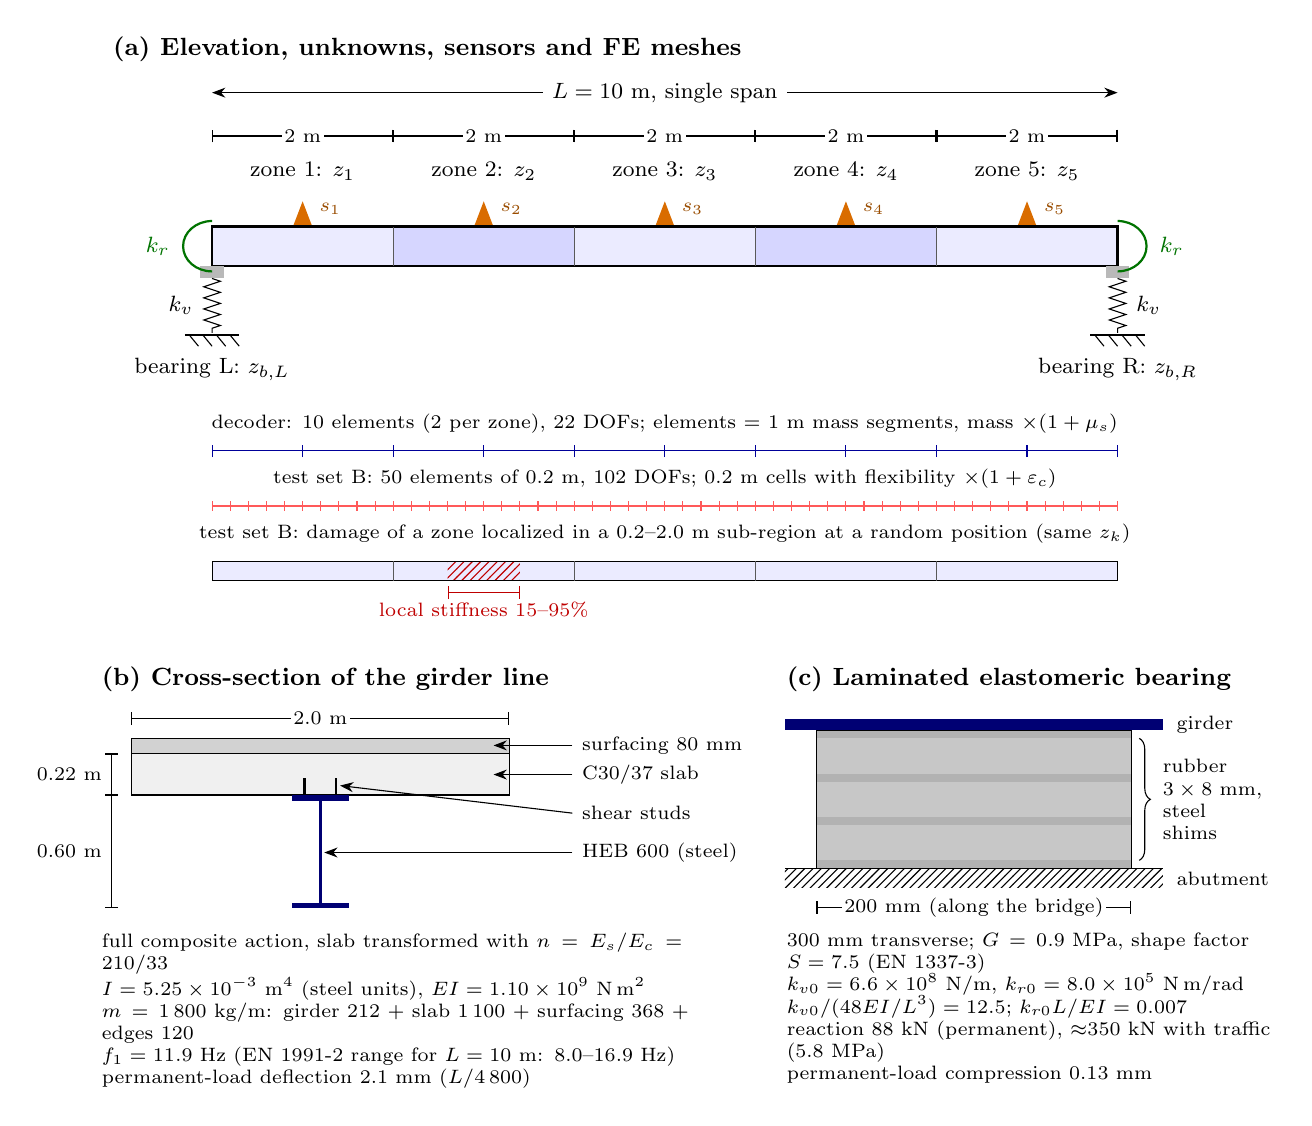
\begin{tikzpicture}[>=Stealth,font=\small]
  % ---------------- (a) Elevation: zones, sensors, bearings, meshes ----------------
  \begin{scope}[x=1.15cm,y=1cm,shift={(1.5,0)}]
  \node[anchor=west,font=\bfseries\small] at (-1.2,2.75) {(a) Elevation, unknowns, sensors and FE meshes};
  \foreach \i/\c in {0/blue!8,1/blue!16,2/blue!8,3/blue!16,4/blue!8}{
    \fill[\c] (2*\i,0) rectangle (2*\i+2,0.5);
    \node[font=\footnotesize] at (2*\i+1,1.2) {zone \the\numexpr\i+1\relax: $z_{\the\numexpr\i+1\relax}$};
    \draw[|-|] (2*\i,1.65) -- (2*\i+2,1.65) node[midway,fill=white,font=\scriptsize,inner sep=1pt] {2 m};
  }
  \draw[thick] (0,0) rectangle (10,0.5);
  \foreach \x in {2,4,6,8} \draw[gray!70!black] (\x,0) -- (\x,0.5);
  \draw[<->] (0,2.2) -- (10,2.2) node[midway,fill=white,font=\footnotesize] {$L=10$ m, single span};
  \foreach \x/\k in {1/1,3/2,5/3,7/4,9/5}{
    \fill[orange!85!black] (\x-0.1,0.52) -- (\x+0.1,0.52) -- (\x,0.82) -- cycle;
    \node[font=\scriptsize,orange!60!black,anchor=west] at (\x+0.08,0.72) {$s_{\k}$};
  }
  \foreach \x/\lab/\a/\b in {0/{L}/90/270,10/{R}/-90/90}{
    \fill[gray!55] (\x-0.13,-0.16) rectangle (\x+0.13,0);
    \draw[decorate,decoration={zigzag,segment length=4,amplitude=3}] (\x,-0.16) -- (\x,-0.85);
    \draw[thick] (\x-0.3,-0.88) -- (\x+0.3,-0.88);
    \foreach \h in {-0.25,-0.1,0.05,0.2} \draw (\x+\h,-0.88) -- (\x+\h+0.1,-1.02);
    \draw[thick,green!45!black] (\x,0.25) ++(\a:0.32) arc (\a:\b:0.32);
    \node[font=\footnotesize,anchor=north] at (\x,-1.05) {bearing \lab: $z_{b,\lab}$};
  }
  \node[anchor=east,font=\footnotesize] at (-0.1,-0.5) {$k_v$};
  \node[anchor=east,green!45!black,font=\footnotesize] at (-0.36,0.25) {$k_r$};
  \node[anchor=west,font=\footnotesize] at (10.1,-0.5) {$k_v$};
  \node[anchor=west,green!45!black,font=\footnotesize] at (10.36,0.25) {$k_r$};
  % decoder mesh
  \node[font=\scriptsize,anchor=south] at (5,-2.25) {decoder: 10 elements (2 per zone), 22 DOFs; elements = 1~m
    mass segments, mass $\times(1+\mu_s)$};
  \draw[blue!60!black] (0,-2.35) -- (10,-2.35);
  \foreach \k in {0,...,10} \draw[blue!60!black] (\k,-2.43) -- (\k,-2.27);
  % test-B mesh
  \node[font=\scriptsize,anchor=south] at (5,-2.95) {test set B: 50 elements of 0.2~m, 102 DOFs; 0.2~m cells
    with flexibility $\times(1+\varepsilon_c)$};
  \draw[red!65] (0,-3.05) -- (10,-3.05);
  \foreach \k in {0,...,50} \draw[red!65] (\k*0.2,-3.11) -- (\k*0.2,-2.99);
  % localized damage of test B
  \node[font=\scriptsize,anchor=south] at (5,-3.65) {test set B: damage of a zone localized in a 0.2--2.0~m
    sub-region at a random position (same $z_k$)};
  \fill[blue!8] (0,-4.00) rectangle (10,-3.75);
  \fill[pattern=north east lines,pattern color=red!75!black] (2.6,-4.00) rectangle (3.4,-3.75);
  \draw (0,-4.00) rectangle (10,-3.75);
  \foreach \x in {2,4,6,8} \draw[gray!70!black] (\x,-4.00) -- (\x,-3.75);
  \draw[|-|,red!75!black] (2.6,-4.15) -- (3.4,-4.15) node[midway,below,font=\scriptsize] {local stiffness 15--95\%};
  \end{scope}
  % ---------------- (b) Cross-section (scale 2.4 cm/m) ----------------
  \begin{scope}[shift={(0.7,-6.0)}]
  \node[anchor=west,font=\bfseries\small] at (-0.5,0.75) {(b) Cross-section of the girder line};
  \fill[gray!35] (0,0) rectangle (4.8,-0.192);
  \fill[gray!12] (0,-0.192) rectangle (4.8,-0.72);
  \draw (0,0) rectangle (4.8,-0.192) (0,-0.192) rectangle (4.8,-0.72);
  \fill[blue!45!black] (2.04,-0.792) rectangle (2.76,-0.72);
  \fill[blue!45!black] (2.382,-2.088) rectangle (2.418,-0.792);
  \fill[blue!45!black] (2.04,-2.16) rectangle (2.76,-2.088);
  \foreach \x in {2.2,2.6} \draw[thick] (\x,-0.72) -- (\x,-0.5);
  \draw[|-|] (0,0.25) -- (4.8,0.25) node[midway,fill=white,font=\scriptsize,inner sep=1pt] {2.0 m};
  \draw[|-|] (-0.25,-0.192) -- (-0.25,-0.72) node[midway,left,font=\scriptsize] {0.22 m};
  \draw[|-|] (-0.25,-0.72) -- (-0.25,-2.16) node[midway,left,font=\scriptsize] {0.60 m};
  \draw[->] (5.6,-0.09) node[right,font=\scriptsize] {surfacing 80 mm} -- (4.6,-0.09);
  \draw[->] (5.6,-0.46) node[right,font=\scriptsize] {C30/37 slab} -- (4.6,-0.46);
  \draw[->] (5.6,-0.95) node[right,font=\scriptsize] {shear studs} -- (2.65,-0.6);
  \draw[->] (5.6,-1.45) node[right,font=\scriptsize] {HEB 600 (steel)} -- (2.45,-1.45);
  \node[anchor=north west,align=left,font=\scriptsize,text width=7.8cm] at (-0.5,-2.35) {%
    full composite action, slab transformed with $n=E_s/E_c=210/33$\\
    $I=5.25\times10^{-3}$ m$^4$ (steel units), $EI=1.10\times10^{9}$ N\,m$^2$\\
    $m=1\,800$ kg/m: girder 212 + slab 1\,100 + surfacing 368 + edges 120\\
    $f_1=11.9$ Hz (EN 1991-2 range for $L=10$ m: 8.0--16.9 Hz)\\
    permanent-load deflection 2.1 mm ($L/4\,800$)};
  \end{scope}
  % ---------------- (c) Laminated elastomeric bearing (1 cm = 50 mm) ----------------
  \begin{scope}[shift={(9.2,-6.0)}]
  \node[anchor=west,font=\bfseries\small] at (-0.3,0.75) {(c) Laminated elastomeric bearing};
  \fill[blue!45!black] (-0.2,0.1) rectangle (4.6,0.25);
  \node[font=\scriptsize,anchor=west] at (4.65,0.175) {girder};
  \fill[gray!60] (0.2,0.1) rectangle (4.2,0);
  \foreach \y in {0,-0.55,-1.1} \fill[black!22] (0.2,\y) rectangle (4.2,\y-0.45);
  \foreach \y in {-0.45,-1.0} \fill[gray!60] (0.2,\y) rectangle (4.2,\y-0.1);
  \fill[gray!60] (0.2,-1.55) rectangle (4.2,-1.65);
  \draw (0.2,0.1) rectangle (4.2,-1.65);
  \fill[pattern=north east lines] (-0.2,-1.65) rectangle (4.6,-1.9);
  \draw (-0.2,-1.65) -- (4.6,-1.65);
  \node[font=\scriptsize,anchor=west] at (4.65,-1.78) {abutment};
  \draw[decorate,decoration={brace,amplitude=4pt}] (4.3,0) -- (4.3,-1.55)
    node[midway,right=5pt,font=\scriptsize,align=left] {rubber\\$3\times8$ mm,\\steel\\shims};
  \draw[|-|] (0.2,-2.15) -- (4.2,-2.15) node[midway,fill=white,font=\scriptsize,inner sep=1pt] {200 mm (along the bridge)};
  \node[anchor=north west,align=left,font=\scriptsize,text width=6.2cm] at (-0.3,-2.35) {%
    300 mm transverse; $G=0.9$ MPa, shape factor $S=7.5$ (EN 1337-3)\\
    $k_{v0}=6.6\times10^{8}$ N/m, $k_{r0}=8.0\times10^{5}$ N\,m/rad\\
    $k_{v0}/(48EI/L^3)=12.5$; $k_{r0}L/EI=0.007$\\
    reaction 88 kN (permanent), $\approx$350 kN with traffic (5.8 MPa)\\
    permanent-load compression 0.13 mm};
  \end{scope}
\end{tikzpicture}
\caption{Revised case study: girder line of a single-span steel--concrete composite bridge on laminated elastomeric
bearings. (a) The seven unknowns are the stiffness reduction factors of the five 2~m deck zones ($z_1,\dots,z_5$, which
scale the bending stiffness of the zone) and of the two bearings ($z_{b,L}$, $z_{b,R}$, which scale both springs of each
bearing), all in $[0.45,1]$. Five vertical accelerometers ($s_1,\dots,s_5$, at $x=1,3,5,7,9$~m) identify the first five
bending modes (2.5\% noise on the frequencies, 5\% of the peak amplitude on the mode shapes). Every measurement comes
from an as-built structure that the nominal decoder does not know: the mass of each 1~m segment is multiplied by
$1+\mu_s$, $\mu_s\sim\mathcal{N}(0,0.05^2)$, and the flexibility of each 0.2~m cell by $1+\varepsilon_c$,
$\varepsilon_c\sim\mathcal{N}(0,0.025^2)$ with zero mean in each zone. Test set B is computed with a 50-element model
and localized damage. (b) Cross-section of the deck. (c) Bearing design. The
rotational springs are drawn in green.}
\label{fig:bridge}
\end{figure}

\begin{table}[H]
\centering\small
\caption{Main specifications of the revised case study.}
\label{tab:specs}
\begin{tabular}{p{3.9cm}p{11cm}}
\toprule
Deck & girder line of a steel--concrete composite deck: HEB~600 + $2.0\times0.22$ m C30/37 slab (full interaction);
$L=10$ m, $EI=1.10\times10^{9}$ N\,m$^2$, mass 1\,800 kg/m (girder, slab, 80 mm surfacing, edges) \\
Bearings (each end) & laminated elastomeric pad (EN~1337-3), $200\times300$ mm, $3\times8$ mm rubber, $G=0.9$ MPa,
shape factor 7.5: $k_{v0}=6.6\times10^{8}$ N/m, $k_{r0}=8.0\times10^{5}$ N\,m/rad \\
Unknowns (latent space) & $\z\in[0.45,1]^7$: five deck zones and two bearings \\
Decoder model & 10 elements (2 per zone), 22 DOFs, nominal mass \\
Data-generating models & as-built structures computed with 10 elements (training, validation and first test set) and
with 50 elements and damage localized inside the zones (second test set), 102 DOFs \\
Observations & first five frequencies (11.91, 42.95, 81.14, 120.80 and 175.48 Hz for the healthy bridge) and vertical
mode shapes at five sensors \\
Measurement noise & 2.5\% on the frequencies; 5\% of the peak amplitude on the mode-shape components \\
Modelling error & mass of each 1 m segment: $\mathcal{N}(0,0.05^2)$; flexibility of each 0.2 m cell:
$\mathcal{N}(0,0.025^2)$ with zero mean in each zone; second test set: finer discretization and localized damage \\
\bottomrule
\end{tabular}
\end{table}

\begin{action}
New description of the case study \lines{xx--yy}, new Fig.~\tbd{x} (Fig.~\ref{fig:bridge}) and new Table~\tbd{x}
(Table~\ref{tab:specs}); all results recomputed with the new datasets \lines{xx--yy}.
\end{action}

% =============================================================================
\section{Reviewer \#1}
% =============================================================================

\begin{rcomment}{}
This paper presents a physics-informed Gaussian copula variational autoencoder for uncertainty-aware damage
identification using noisy natural frequencies and mode shapes. Replacing the learned decoder with a differentiable
eigensolver appears to be an interesting approach for end-to-end training, and the manuscript is clearly written. The work
builds on the authors' earlier Gaussian copula VAE (Reference 41) and extends it by embedding the eigensolver and
increasing the latent dimensionality from 2 to 5. The current validation is based on a single five-element synthetic
beam with measurement noise, and I believe that some additional evidence would further strengthen the conclusions
regarding uncertainty quantification, reliability, and scalability. Some clarifications are needed to better understand
the method and its applications.
\end{rcomment}

\begin{response}
We thank the reviewer for the positive assessment and for the constructive comments. Following them, the revised
study is no longer based on a single five-element beam with measurement noise: the structure is a girder line of a
short-span composite bridge on elastomeric bearings, the latent space has seven variables, the data include modelling
errors, and the trained model is tested on data from two FE models. The responses below describe these changes.
\end{response}

% -----------------------------------------------------------------------------
\begin{rcomment}{1}
The training and test data are generated using the same five-element model. Could the authors consider testing the
trained model on observations generated from a finer mesh while retaining the same five damage zones and sensor
locations as in the current paper? This would help assess robustness to model-form uncertainty, since field observations
may not necessarily be well represented by such a coarse discretization.
\end{rcomment}

\begin{response}
We agree that generating training and test data with the model embedded in the decoder is a favourable setting, and
we have followed the reviewer's suggestion.

\textit{Decoder model.} Before testing on finer-mesh data, we checked whether the model embedded in the decoder is
accurate enough. With respect to the 50-element model of the second test set, one element per zone (the discretization
of the submitted version) gives errors of 0.9\% and 1.4\% on the fourth and fifth frequencies (Table~\ref{tab:mesh}),
about half of the identification noise, so a finer-mesh test would partly measure the discretization error of the
decoder. We therefore embed a 10-element model (two elements per zone) in the decoder; its error is below 0.13\% for the
five modes used. The latent variables are still one stiffness factor per damage zone (plus one per bearing, see R2.2),
whatever the number of elements:
\begin{equation}
\hat{\mathbf{K}}_{\mathrm{G}}(\z)=\sum_{k=1}^{5} z_k\sum_{e\in\mathcal{Z}_k}\mathbf{K}_{e}
+z_{b,L}\,\mathbf{K}_{b,L}+z_{b,R}\,\mathbf{K}_{b,R},
\label{eq:Kz}
\end{equation}
where $\mathcal{Z}_k$ is the set of elements of zone $k$ and $\mathbf{K}_{b,L}$, $\mathbf{K}_{b,R}$ contain the nominal
bearing springs.

\textit{Two test sets with the same damage conditions.} The test set contains 1\,200 as-built structures (damage
condition and as-built deviations, see R1.2), observed twice with the same measurement-noise realizations. Test set A is
computed with the 10-element model (the discretization of the decoder). Test set B is computed with a 50-element model
(ten elements per zone), with the same five damage zones and the same five sensors. Because a finer mesh alone changes
the modal data very little (Table~\ref{tab:budget}), test set B also represents the damage more realistically: in every
damaged zone, the loss of stiffness is concentrated in a sub-region of random length (0.2--2.0~m, median 1.2~m) and
position, with the same equivalent (harmonic-mean) stiffness $z_k$ of the zone (R2.3). The decoder can represent
neither the finer mesh nor the localization, so test set B measures the robustness to model-form error. The sensors are
placed at the zone centres instead of the zone boundaries (see R3.4).

\textit{Results so far.}
\begin{itemize}[leftmargin=*]
\item The finer mesh alone shifts the frequencies by at most $-0.13\%$ (mode 5) and leaves the mode shapes at the sensors
unchanged ($1-\mathrm{MAC}<10^{-5}$). The localized damage changes the frequencies by 0.7--1.6\% (standard deviation over
the test damage states) and the mode shapes by up to $2.4\times10^{-3}$ in $1-\mathrm{MAC}$: an error of the same order
as that of the mass deviations (Table~\ref{tab:budget}).
\item The likelihood is calibrated on test set A: at the true damage condition, the frequency term equals 1.02 times its
theoretical value and the mode-shape terms 0.98--1.01 times. On test set B these ratios are 1.15 and 1.00--1.32,
because the likelihood does not include the localization (Fig.~\ref{fig:calib}): test set B is a genuine case of model
misspecification.
\item The exact posteriors (sequential Monte Carlo, see R1.3) of the 11 benchmark scenarios contain the true damage
condition in their 95\% credible intervals for 68 (test set A) and 69 (test set B) of the 77 parameters. For seven
benchmarks (P0--P4, P9 and P10), the posteriors from both test sets are almost identical (means within 0.035); for
P5--P8, the localization changes the posterior means by 0.06--0.24 and the standard deviations by up to 47\%. The largest
change occurs in P5, where the damage of zone 1 is combined with that of the left bearing: the localized damage changes
how the data distribute the loss of stiffness between the end zone and the bearing (Fig.~\ref{fig:testfine}).
\item VAE metrics on both test sets: \tbd{Table with MSE, MAE, ALL, MACE and coverage on test sets A and B}.
\end{itemize}
\end{response}

\begin{table}[H]
\centering\small
\caption{Relative error (\%) of the natural frequencies of the healthy bridge with respect to the 50-element model of
the second test set.}
\label{tab:mesh}
\begin{tabular}{lccccc}
\toprule
Model & $f_1$ & $f_2$ & $f_3$ & $f_4$ & $f_5$ \\
\midrule
5 elements (discretization of the submitted version) & 0.010 & 0.131 & 0.464 & 0.898 & 1.360 \\
10 elements (decoder) & 0.001 & 0.008 & 0.029 & 0.063 & 0.125 \\
\midrule
Frequencies of the 50-element model [Hz] & 11.906 & 42.950 & 81.114 & 120.729 & 175.263 \\
\bottomrule
\end{tabular}
\end{table}

\begin{figure}[H]
\centering
\begin{subfigure}{0.49\textwidth}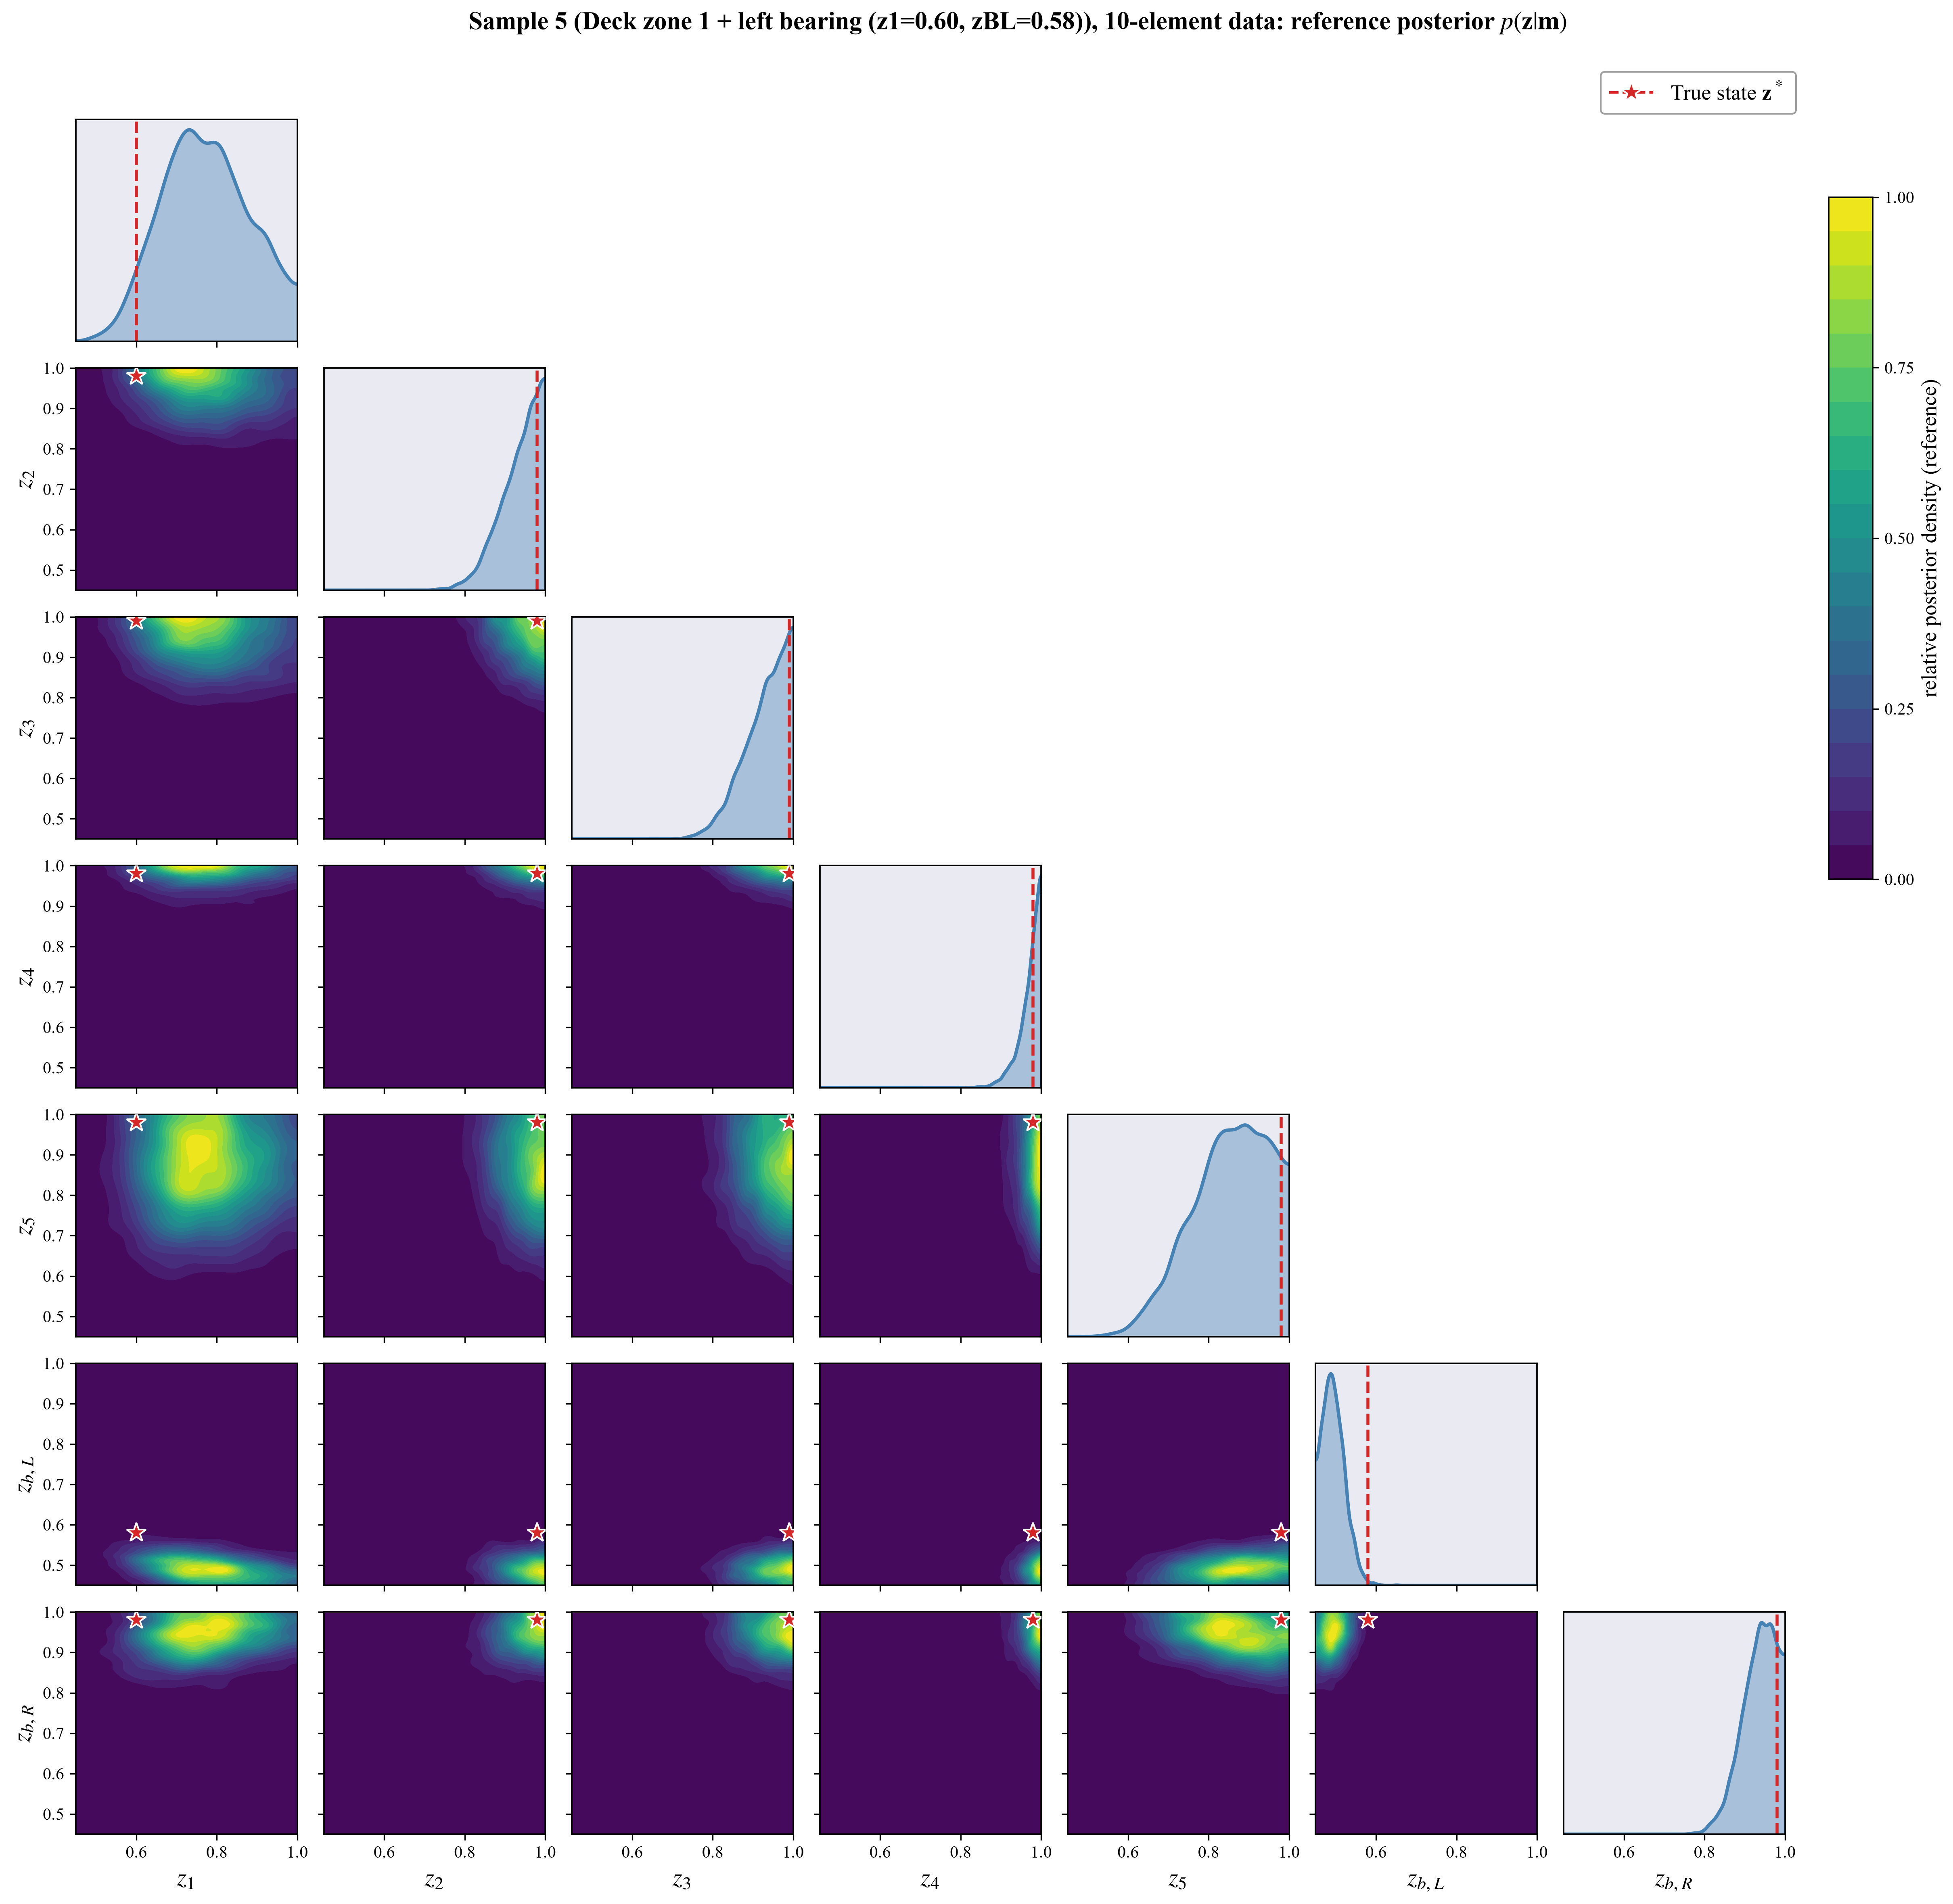
\includegraphics[width=\textwidth]{figures_final/Fig_reference_posterior_P5_test.png}
\caption{Test set A: 10-element model, uniform damage of zone 1}\end{subfigure}
\begin{subfigure}{0.49\textwidth}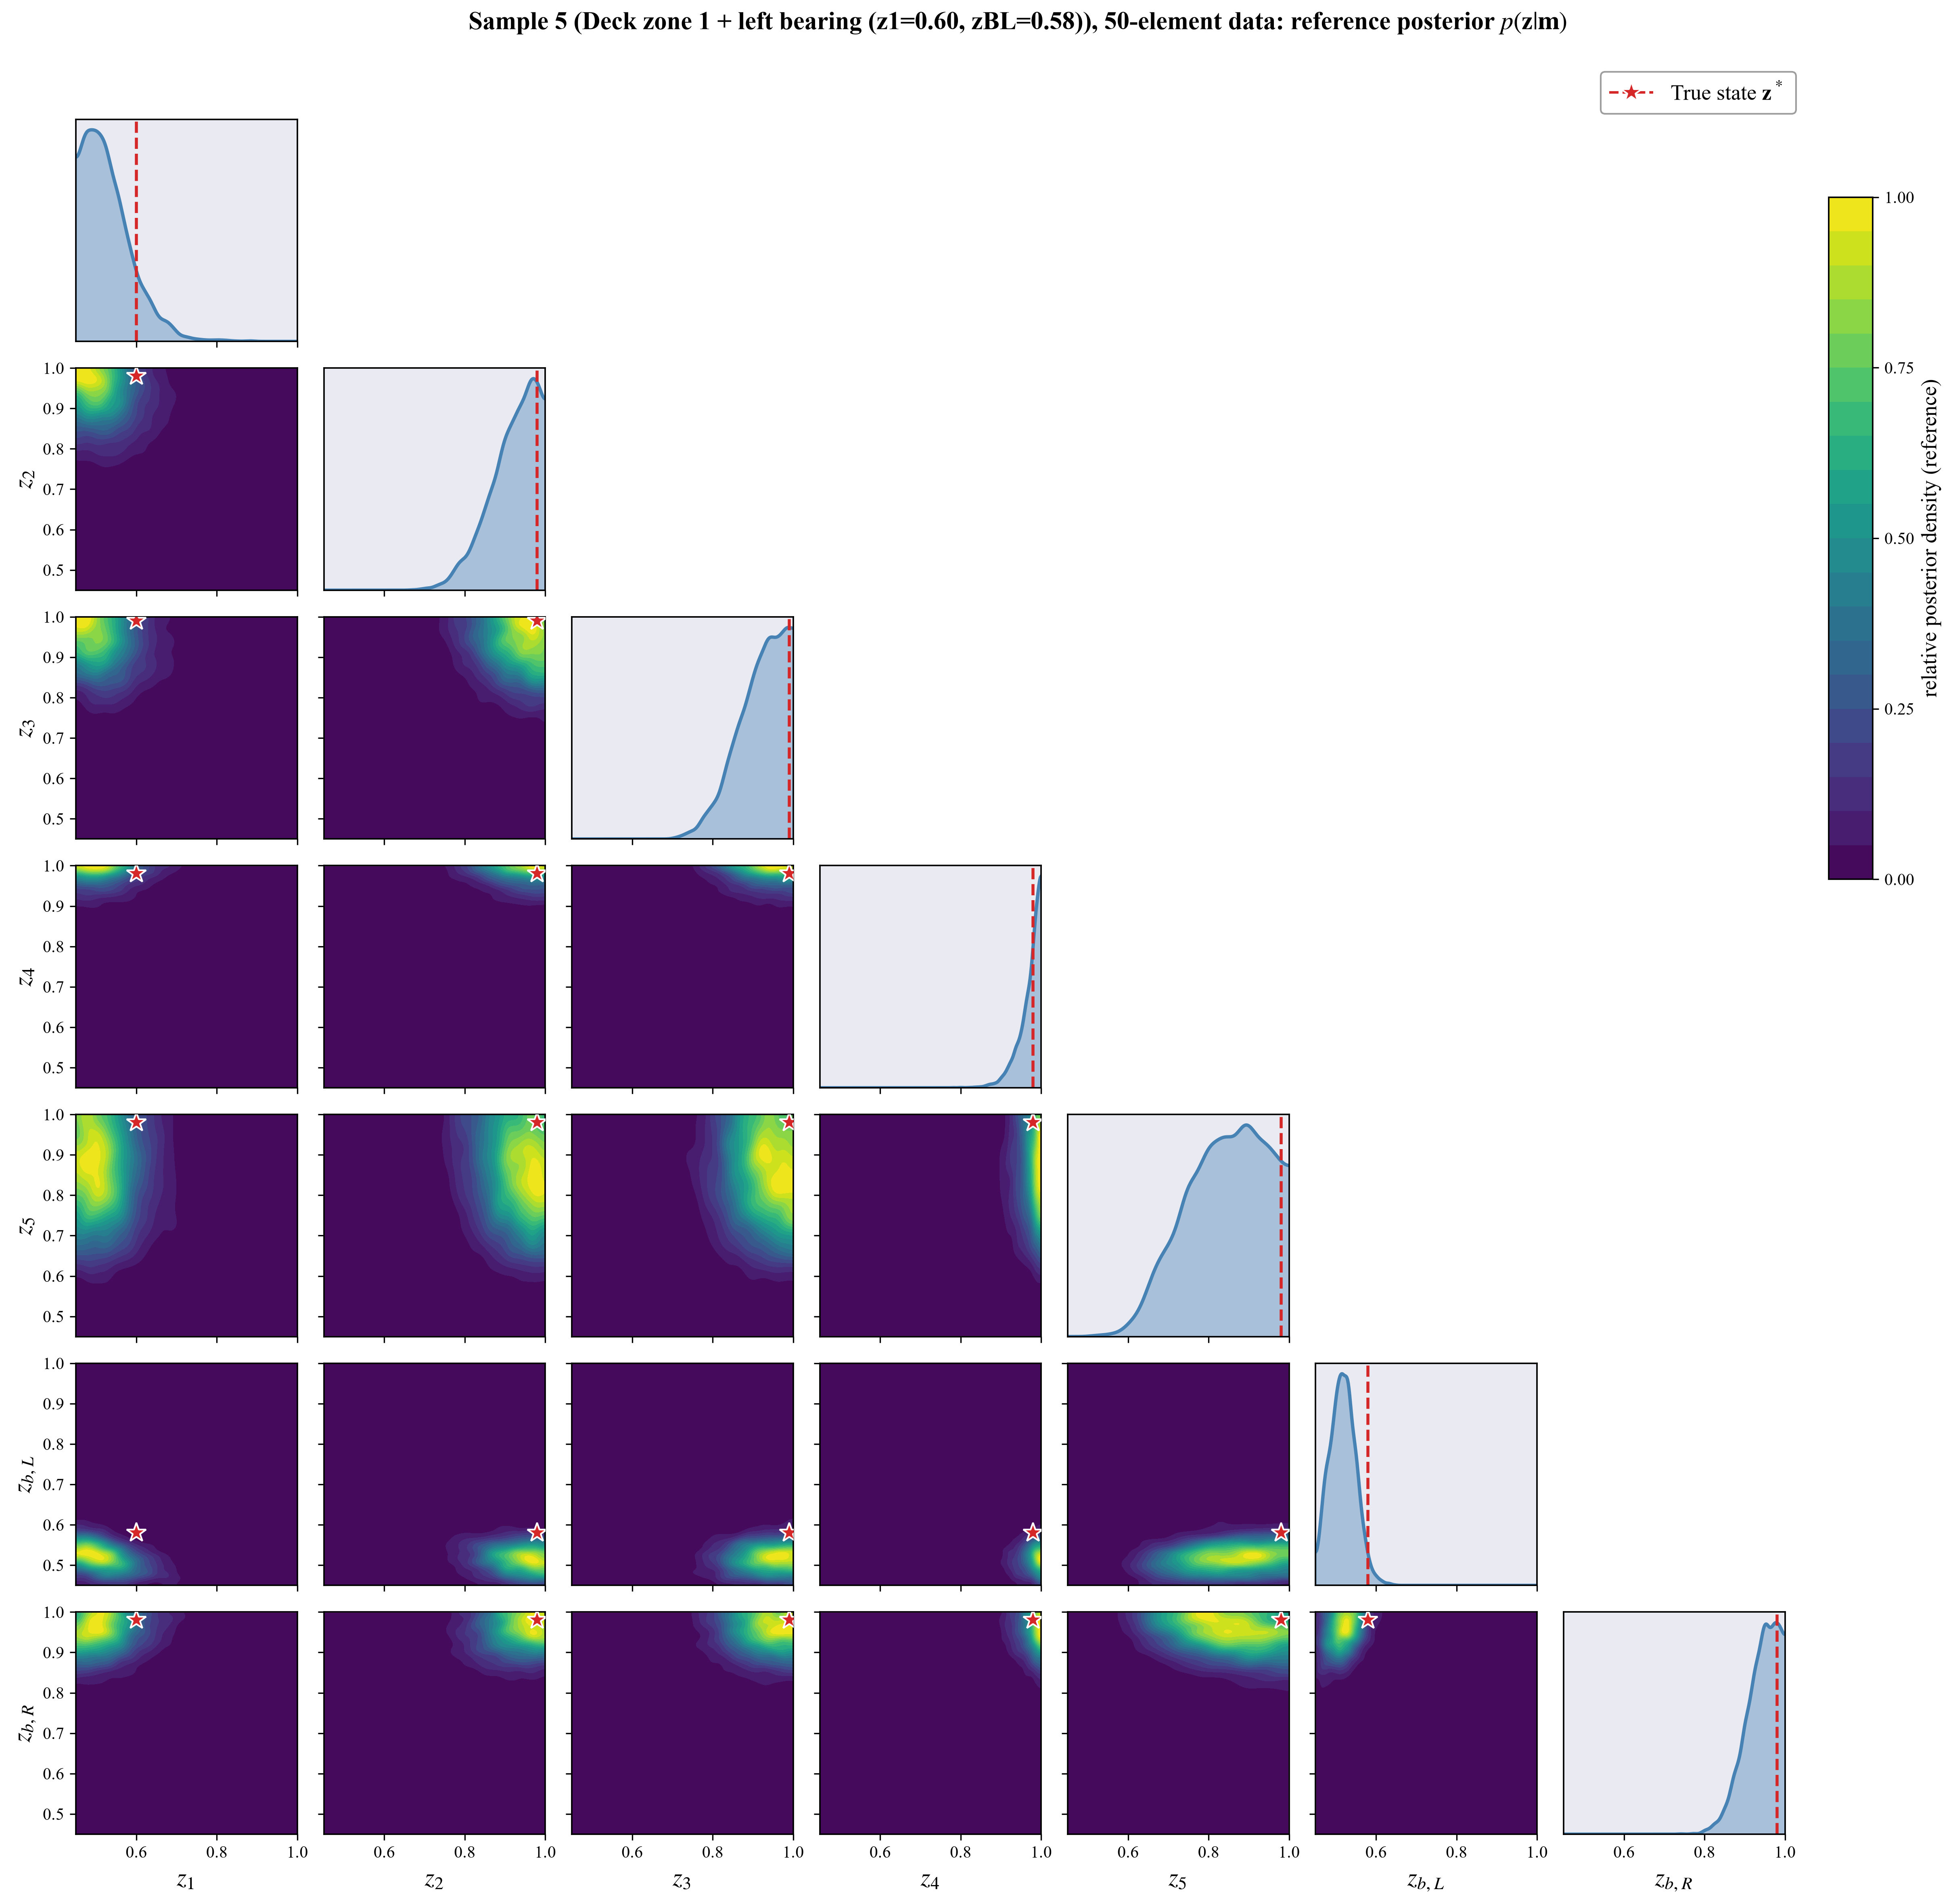
\includegraphics[width=\textwidth]{figures_final/Fig_reference_posterior_P5_test_fine.png}
\caption{Test set B: 50-element model, localized damage of zone 1}\end{subfigure}
\caption{Exact posterior of benchmark P5 (zone 1 and left bearing damaged, $z_1=0.60$, $z_{b,L}=0.58$) computed from the
observations of the two test sets (same damage condition, as-built deviations and noise realization). The red stars mark
the true damage condition.}
\label{fig:testfine}
\end{figure}

\begin{action}
The decoder now embeds a 10-element model \lines{xx--yy}; a second test set generated with a 50-element model and
localized damage is described in \lines{xx--yy}, and Table~\tbd{x} reports the metrics on both test sets.
\end{action}

% -----------------------------------------------------------------------------
\begin{rcomment}{2}
The introduction identifies model uncertainty, measurement error, and environmental variability as sources of
ill-posedness, whereas the numerical study focuses primarily on measurement noise. It would be useful to investigate how
the proposed framework handles the other sources of uncertainty or, alternatively, to discuss this point more explicitly
as a limitation of the present study.
\end{rcomment}

\begin{response}
We agree. The revised study includes, in every dataset (training, validation and both test sets), the two sources of
uncertainty that can be represented realistically in a synthetic setting: measurement error and modelling error.

\textit{Measurement error.} As in the submitted version, we add 2.5\% noise to the identified frequencies and noise with
a standard deviation of 5\% of the peak amplitude to each mode-shape component.

\textit{Modelling error.} Each measurement comes from an as-built structure that differs from the nominal FE model
embedded in the decoder:
\begin{itemize}[leftmargin=*]
\item \emph{Mass}: the mass of each 1 m segment is multiplied by $1+\mu_s$, with $\mu_s\sim\mathcal{N}(0,0.05^2)$
(non-structural mass, pavement, tolerances of the cross-sections).
\item \emph{Stiffness variability within each zone}: the flexibility of each 0.2 m cell is multiplied by
$1+\varepsilon_c$, with $\varepsilon_c\sim\mathcal{N}(0,0.025^2)$ and zero mean inside each zone, so that the
equivalent stiffness of the zone remains $z_k$.
\item \emph{Discretization and damage morphology} (second test set only): 50-element model in which the damage of each
damaged zone is concentrated in a sub-region of the zone (R1.1, R2.3).
\end{itemize}
The element matrices of an as-built structure are therefore
\begin{equation}
\mathbf{M}_e^{\mathrm{ab}}=(1+\mu_{s(e)})\,\mathbf{M}_e,\qquad
\mathbf{K}_e^{\mathrm{ab}}=\frac{z_{k(e)}}{1+\bar{\varepsilon}_e}\,\mathbf{K}_e ,
\label{eq:asbuilt}
\end{equation}
where $s(e)$ is the segment and $k(e)$ the zone of element $e$, and $\bar{\varepsilon}_e$ is the mean flexibility
deviation of the cells of the element. Since the deviations are defined on a grid that does not depend on the mesh,
both test sets describe the same physical structures. The decoder keeps the nominal model: the realizations of these
deviations are never available to the VAE.

\textit{How the inference handles them.} We write the observations as
\begin{equation}
\m=\mathbf{g}(\z)+\bm{\delta}_{\mathrm{model}}+\bm{\epsilon}_{\mathrm{meas}},
\label{eq:discrepancy}
\end{equation}
where $\mathbf{g}(\z)$ are the modal properties of the nominal model. If the likelihood ignored
$\bm{\delta}_{\mathrm{model}}$, the stiffness factors would have to absorb the modelling error, which biases the
estimates and makes the posterior overconfident. Instead, we estimate the statistics of
$\bm{\delta}_{\mathrm{model}}+\bm{\epsilon}_{\mathrm{meas}}$ by simulating 6\,000 as-built structures with new random
deviations, and include them in the likelihood: a full covariance matrix of the log-frequency errors (standard
deviations 2.66--2.72\%, of which 0.9--1.1\% is due to the modelling error; correlations between modes below 0.13) and
a standard deviation per mode for the mode-shape errors (0.028--0.044). This is the standard treatment of model
discrepancy in Bayesian FE model updating, and it leaves the architecture unchanged. We verified the calibration on
independent data generated like the training data (test set A): at the true damage condition, every likelihood term
equals 0.98--1.02 times its theoretical value. On test set B, whose localized damage is not included in the likelihood,
the ratios are 1.00--1.32 (Fig.~\ref{fig:calib}). Table~\ref{tab:budget} and Fig.~\ref{fig:budget} quantify each
source: the mass deviations are the dominant modelling error of the training data (about 1\% on the frequencies and up to
$3.3\times10^{-3}$ in $1-\mathrm{MAC}$ for mode~5); in test set B, the localized damage adds an error of similar size
(0.7--1.6\% on the frequencies), while the finer mesh alone only introduces a small systematic shift (at most 0.13\%).

\textit{Environmental variability.} We do not simulate environmental effects. Their influence on the modal properties
depends strongly on the structure (for instance, the stiffening of the pavement and of the bearings below freezing), and
a realistic description requires long-term monitoring data with measured temperatures. We now discuss this explicitly
as a limitation. The framework can incorporate such effects either as an additional, correlated term of
$\bm{\delta}_{\mathrm{model}}$ in Eq.~\eqref{eq:discrepancy}, or by feeding the measured temperature to the encoder; we
indicate this as future work with field data.
\end{response}

\begin{table}[H]
\centering\small
\caption{Size of each source of discrepancy between the measurements and the nominal decoder (modes 1 to 5), over the
damage states of the design of experiments: mean and standard deviation of $\log f_{\mathrm{data}}-\log
f_{\mathrm{decoder}}$ and mean $1-\mathrm{MAC}$ of the vertical mode shapes (range over the five modes).}
\label{tab:budget}
\begin{tabular}{lccc}
\toprule
Source & Mean $\Delta\log f$ (\%) & Std $\Delta\log f$ (\%) & Mean $1-\mathrm{MAC}$ \\
\midrule
Finer mesh (50 elements) & $-0.001$ to $-0.129$ & $\le0.010$ & $<10^{-5}$ \\
Mass (5\% per 1 m segment) & 0.003 to 0.051 & 0.91--1.09 & up to $3.3\times10^{-3}$ \\
Within-zone stiffness (2.5\%) & $\le0.001$ & 0.03--0.08 & $<10^{-5}$ \\
Localized damage (test set B) & $-0.07$ to 0.08 & 0.74--1.58 & up to $2.4\times10^{-3}$ \\
\midrule
All modelling errors, training and test A & 0.004 to 0.053 & 0.91--1.09 & up to $3.3\times10^{-3}$ \\
All modelling errors, test B & $-0.035$ to 0.107 & 1.20--1.82 & up to $5.6\times10^{-3}$ \\
Measurement noise & $\approx0$ & 2.45--2.53 & 3.0--4.3$\times10^{-3}$ \\
\bottomrule
\end{tabular}
\end{table}

\begin{figure}[H]
\centering
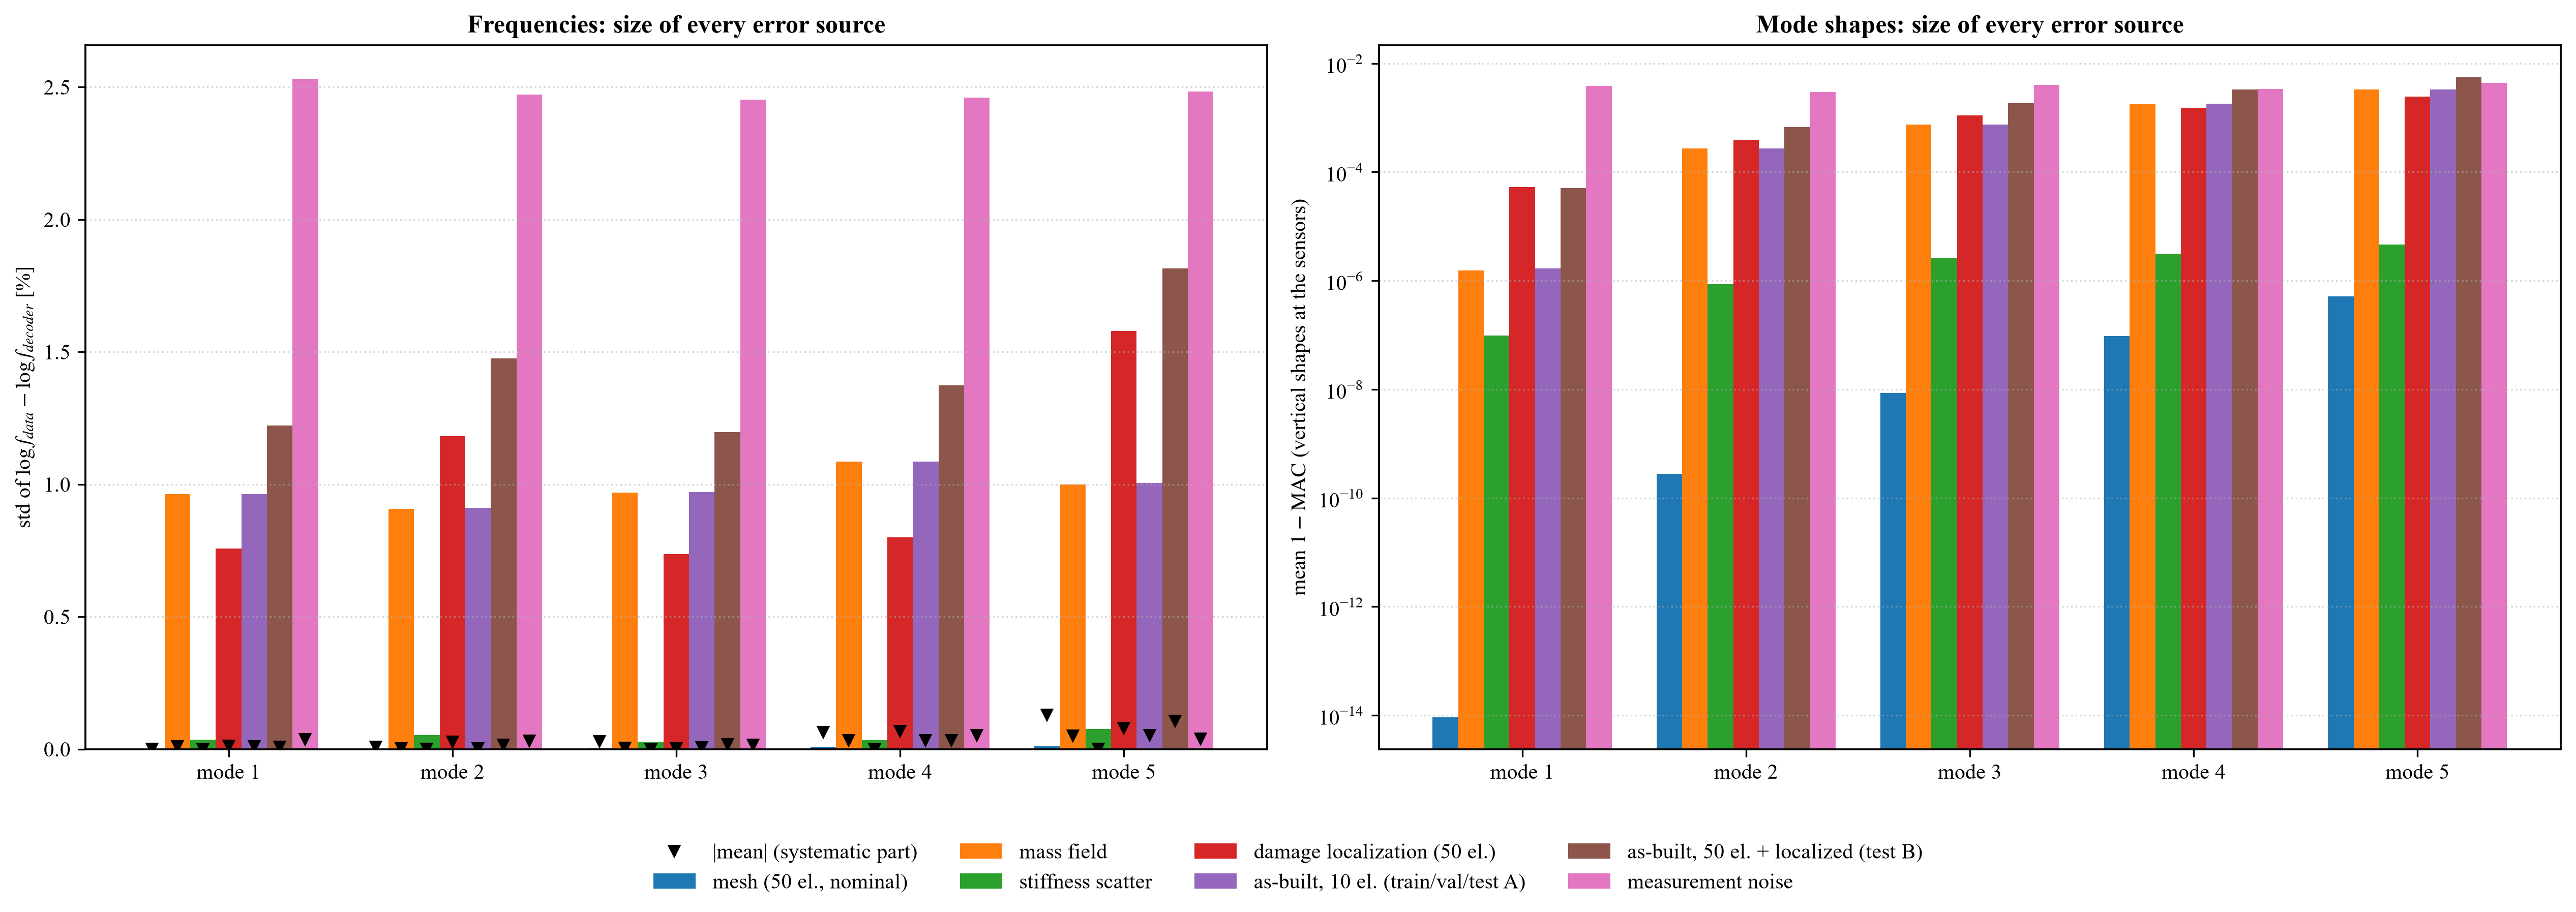
\includegraphics[width=\textwidth]{figures_final/Fig_model_error_budget.png}
\caption{Size of each source of discrepancy between the measurements and the nominal decoder, per mode: frequencies
(left) and vertical mode shapes (right).}
\label{fig:budget}
\end{figure}

\begin{figure}[H]
\centering
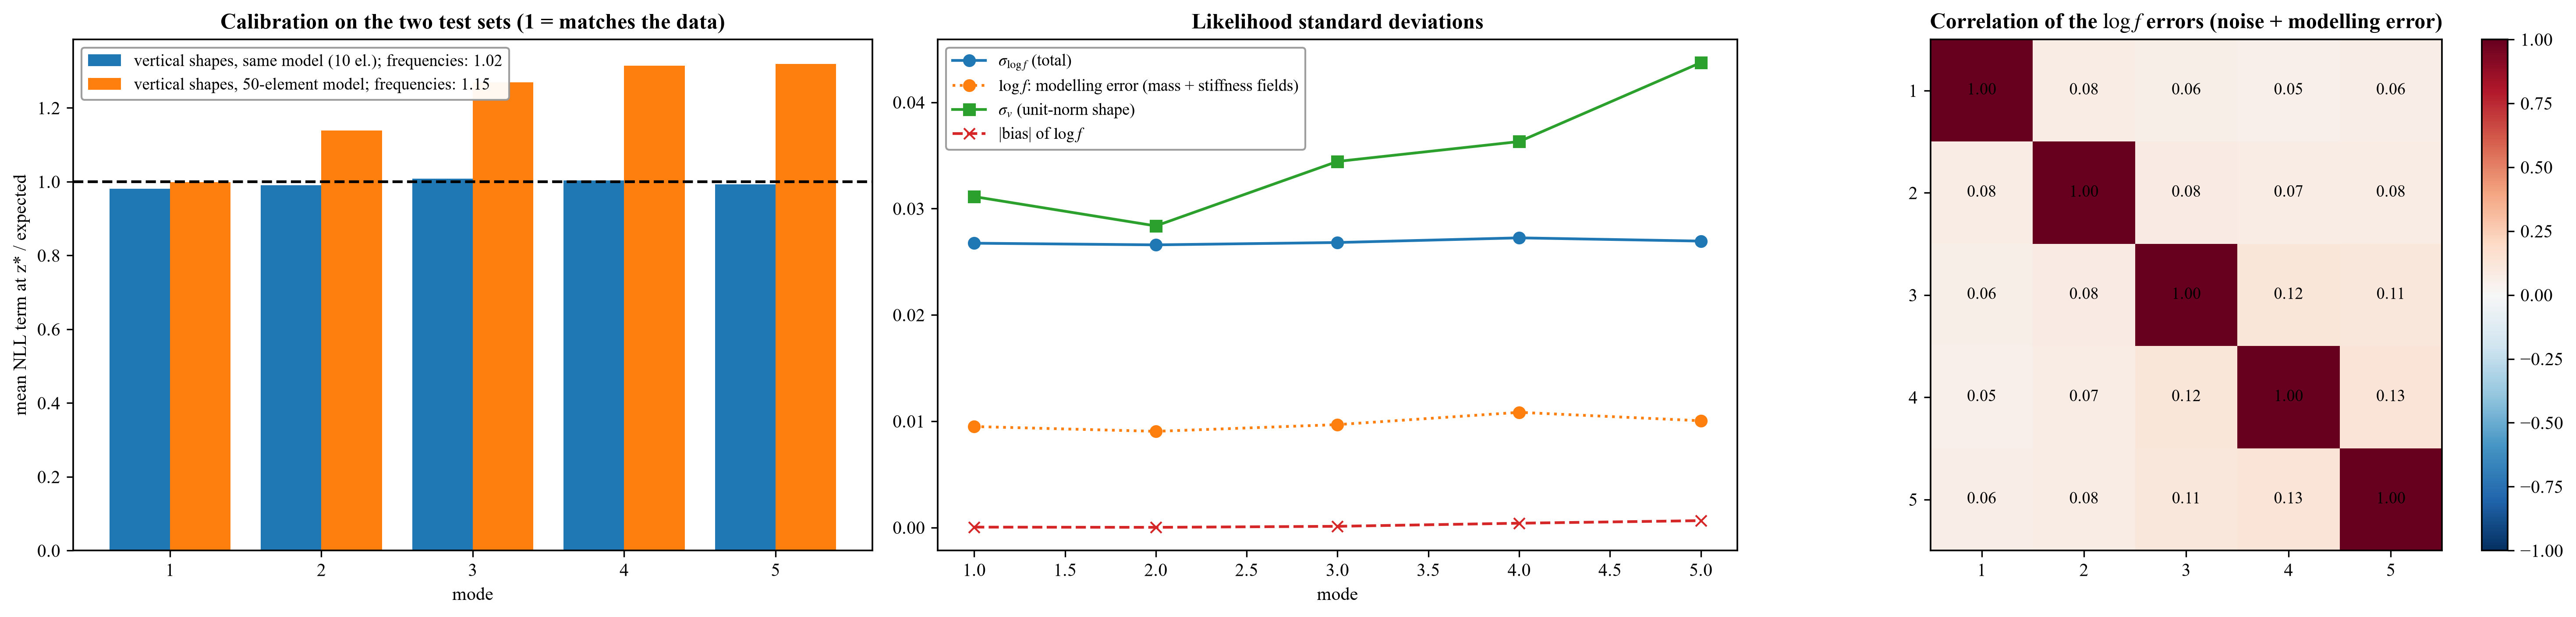
\includegraphics[width=\textwidth]{figures_final/Fig_likelihood_calibration.png}
\caption{Calibration of the likelihood. Left: average likelihood terms at the true damage condition divided by their
theoretical value, for both test sets (1 means calibrated). Centre: standard deviations of the log-frequencies and of
the unit-norm vertical mode shapes. Right: correlation between the log-frequency errors of different modes.}
\label{fig:calib}
\end{figure}

\begin{action}
New subsection on the sources of uncertainty and their treatment in the likelihood \lines{xx--yy}, with
Eqs.~\eqref{eq:asbuilt}--\eqref{eq:discrepancy}, Table~\ref{tab:budget} and Figs.~\ref{fig:budget}--\ref{fig:calib};
environmental variability discussed as a limitation in the conclusions \lines{xx--yy}.
\end{action}

% -----------------------------------------------------------------------------
\begin{rcomment}{3}
The abstract reports 77.2\% coverage (line 32), whereas line 352 reports a value of 0.789 for nominal 95\% intervals.
Could the authors clarify how these two values are related? A value below 80\% for nominal 95\% intervals may indicate
some undercoverage. A brief discussion of how the uncertainty intervals are calibrated would therefore be helpful.
\end{rcomment}

\begin{response}
We thank the reviewer for pointing out this inconsistency. The two values were obtained in two different evaluation
runs of the submitted version, and the abstract was not updated after the final run.
\authornote{please confirm the origin of 77.2\% and 0.789.} In the revised manuscript, a single coverage value is
reported, the abstract and the text use the same value, and the definition of the intervals is stated explicitly.

The reviewer is right that these values indicate undercoverage. We identified two causes:
\begin{enumerate}[leftmargin=*]
\item \emph{The width of the approximate posterior was not calibrated.} In the submitted loss, the frequency and MAC
terms had fixed weights ($\lambda=10$) that were not derived from the noise statistics, and the entropy term was
scaled by $\gamma^2$, with $\gamma=0.30$ selected to balance point accuracy and distributional quality. The minimizer of such a loss is a tempered posterior
whose width depends on these weights, so its credible intervals cannot be expected to reach their nominal coverage.
\item \emph{Equal-tailed intervals and the upper bound $z=1$.} An undamaged parameter lies close to the upper bound of
the support, where its posterior accumulates. An equal-tailed (central) 95\% interval excludes the upper 2.5\% of the
probability, and therefore often excludes a true value close to 1, even when the posterior is correct. In the revised
test set, 67\% of the parameters are undamaged ($z^*\ge0.95$) and 18\% lie above the 97.5\% quantile of the prior. As a
result, even the prior, which ignores the data, reaches only 81\% coverage with central 95\% intervals on this test set.
A coverage of central intervals below 80\% is therefore not necessarily a sign of a poorly calibrated posterior.
\end{enumerate}

We made the following changes:
\begin{itemize}[leftmargin=*]
\item \emph{Calibrated likelihood.} The data terms of the loss are the negative log-likelihood of the frequency and
mode-shape errors, with the variances calibrated by simulation and verified on independent data (R1.2):
\begin{equation}
\mathrm{NLL}(\z;\m)=\tfrac12\,\mathbf{d}^{\top}\bm{\Sigma}_f^{-1}\mathbf{d}
+\sum_{j=1}^{n_m}\frac{1-\mathrm{MAC}_j(\bm{\Phi},\hat{\bm{\Phi}}(\z))}{2\,s_{v,j}^2},\qquad
\mathbf{d}=\log\f-\mathbf{b}-\log\hat{\f}(\z).
\label{eq:nll}
\end{equation}
For unit-norm mode shapes perturbed by Gaussian noise, $1-\mathrm{MAC}_j$ equals the squared noise component
perpendicular to the shape, so the second term is the Gaussian log-likelihood of that component.
\item \emph{No tempering ($\gamma=1$).} With a uniform prior on $\mathcal{S}=[0.45,1]^7$, the loss
\begin{equation}
\mathcal{L}(\bm\theta)=\frac1N\sum_{i=1}^N\Big(\mathbb{E}_{q}\big[\mathrm{NLL}(\z;\m_i)\big]
-\gamma^2\,\mathcal{H}\big[q_{\bm\zeta_{\bm\theta}}(\z|\m_i)\big]\Big)
\label{eq:loss}
\end{equation}
is the negative ELBO for $\gamma=1$ (up to a constant), and its minimizer is the Bayesian posterior within the
variational family. $\mathcal{H}$ is the entropy of the copula model: the copula part, $\frac12\log\det\mathbf{R}$, is
computed exactly, and only the entropies of the marginals are estimated with the samples.
\item \emph{Exact credible intervals.} The marginals of the approximate posterior are Kumaraswamy mixtures with a
closed-form CDF $F_{q,e}$, so we compute the probability integral transform $u_{t,e}=F_{q,e}(z^*_{t,e})$ of every true
value exactly. The true value lies inside the equal-tailed interval of level $p$ if $|2u_{t,e}-1|\le p$, and inside the
highest-density region of level $p$ if the posterior probability of $\{z: q_e(z)>q_e(z^*_{t,e})\}$ does not exceed $p$.
\item \emph{Reliability diagrams.} We compute the empirical coverage at 19 nominal levels, from $p=0.05$ to $p=0.95$ in
steps of 0.05, and the MACE, with both types of intervals, for all parameters and separately for deck zones and bearings, for damaged and
undamaged parameters, and for the test scenarios drawn from the prior, where a Bayesian posterior must be calibrated by
construction.
\item \emph{Reference posterior.} We compare the VAE with the exact posterior obtained by sequential Monte Carlo with
the same likelihood and prior. It starts from samples of the prior, introduces the likelihood gradually through an
exponent that grows from 0 to 1, and never uses the true damage condition. This separates the approximation error of
the VAE from the effect of the bounds described above.
\end{itemize}

\tbd{Results of the final training: coverage and MACE with both types of intervals (all, deck zones, bearings,
damaged, undamaged, scenarios drawn from the prior), reliability diagram, and comparison with the exact posteriors of
the benchmark scenarios.}
\end{response}

\begin{action}
Abstract and Section~\tbd{x} corrected so that they report the same value \lines{xx--yy}; new paragraph on the
calibration of the likelihood and the definition of the intervals \lines{xx--yy}; new reliability diagram (Fig.~\tbd{x})
and coverage table (Table~\tbd{x}).
\end{action}

% -----------------------------------------------------------------------------
\begin{rcomment}{4}
References 39 (Gaussian mixture autoencoder) and 41 (Gaussian copula VAE) introduce closely related methods that could
potentially serve as useful baselines. A comparison with these approaches would help assess the benefits of the proposed
strategy more effectively.
\end{rcomment}

\begin{response}
We agree, and we added both methods as baselines. To isolate the effect of the form of the approximate posterior, the
three models use the same data, the same eigenvalue decoder and calibrated likelihood, the same uniform prior and
negative ELBO ($\gamma=1$), the same encoder layers (three fully connected layers with 128, 256 and 128 units), the same
training schedule and model selection on the validation set, and the same evaluation code. They differ only in the
variational family:
\begin{itemize}[leftmargin=*]
\item \emph{Gaussian copula VAE (Ref.~41, and the submitted version):} Gaussian copula with one Gaussian marginal per
parameter, truncated to the support of the prior. The samples are obtained with the closed-form quantile of the
truncated normal distribution (no rejection sampling), and the entropy of the marginals is computed in closed form.
\item \emph{Gaussian mixture autoencoder (Ref.~39):} a mixture of $K=5$ Gaussians with full covariance matrices and no
copula. To respect the support of the prior, the mixture is defined in the logit space of $[0.45,1]^7$, as in automatic
differentiation variational inference (Kucukelbir et al., 2017); a Gaussian mixture defined directly in $\z$ would place
probability outside the support, where the prior density vanishes. The expectation over the mixture is computed by
stratified sampling over its components (Morningstar et al., 2021), so the mixture weights receive exact gradients.
\item \emph{Proposed model:} Gaussian copula with Kumaraswamy-mixture marginals.
\end{itemize}
The models are compared with the metrics of R1.3 on both test sets, with the agreement with the exact posteriors of the
benchmarks, and with two diagnostics that do not require reference samples. The first is the negative ELBO on the
validation set, which equals the Kullback--Leibler divergence from the exact posterior up to a constant that does not
depend on the model. The second is the Pareto-$\hat{k}$ diagnostic of importance sampling (Yao et al., 2018; Vehtari
et al., 2024), which indicates whether the approximation misses probability mass of the exact posterior.

The same validation criterion selects the number $K$ of Kumaraswamy components of the proposed model (Editor, item 7):
we train $K=1,\dots,5$ with two random seeds and select the smallest $K$ whose validation negative ELBO lies within one
standard error of the best value (one-standard-error rule, Hastie et al., 2009). The test sets are not used for this
choice.
\tbd{Table: proposed model vs.\ baselines (validation negative ELBO, Pareto-$\hat{k}$, MSE, MAE, ALL, MACE and 95\%
coverage on test sets A and B, agreement with the exact posteriors); reliability diagrams; selection of $K$.}
\end{response}
\authornote{code in the folders baseline\_GaussCopula\_GaussMarginals, baseline\_GaussMixture\_K5 and
model\_comparison of MODULES (to be run on the final dataset). Add the references cited in this response.}

\begin{action}
New subsection ``Comparison with related methods'' \lines{xx--yy}, with Table~\tbd{x} and Fig.~\tbd{x}; selection of
the number of Kumaraswamy components \lines{xx--yy}.
\end{action}

% -----------------------------------------------------------------------------
\begin{rcomment}{5}
All test cases appear to be sampled from the same distribution as the training data. It would be helpful to include
several additional cases where the test data fall outside the training distribution to illustrate how the proposed
method behaves under distribution shift.
\end{rcomment}

\begin{response}
We agree. Besides test set B, which already differs from the training data in its FE model and damage morphology (R1.1),
we added six test sets outside the training distribution. Each one changes a single factor with respect to test set B
and, except for the second, contains the same structures and noise realizations, so that every change in the results is
caused by the shift alone. The VAE is not retrained, and the decoder and the likelihood remain those of the training
data:
\begin{enumerate}[leftmargin=*]
\item \emph{Damage beyond the training and prior range}: the damaged deck zones have $z\in[0.30,0.45)$.
\item \emph{Damage not aligned with the zones}: one or two defects of 0.2--0.6~m with the local stiffness reduced to
25--70\% of its nominal value, at random positions, including across zone boundaries and next to the supports.
\item \emph{Noise twice the assumed level}: 5\% on the frequencies and 10\% on the mode shapes.
\item \emph{Modelling error twice the assumed level}: 10\% mass and 5\% stiffness deviations.
\item \emph{Systematic modelling error}: 5\% of additional mass not included in the model (e.g., a new surfacing layer).
\item \emph{Bearings stiffer than nominal} (by a factor of 3, e.g., aged or partially seized pads), outside the support of
the prior.
\end{enumerate}
For each set, we report the metrics of R1.3, the detection and false-alarm rates, and the exact posteriors of 40 cases.
Comparing the VAE with the exact posterior separates two effects: the misspecification of the Bayesian model itself,
which affects any method that uses the same model and likelihood, and the amortization error of the encoder for inputs
that differ from its training data, which we measure with the Pareto-$\hat{k}$ diagnostic and the distance to the exact
posteriors.
\tbd{Results: summary table, reliability diagrams and examples.}
\end{response}
\authornote{code: MODULES/review29oct\_fixed/ood\_study.py (to be run on the final dataset).}

\begin{action}
New subsection on the behaviour under distribution shift \lines{xx--yy}, with Table~\tbd{x} and Fig.~\tbd{x}.
\end{action}

% -----------------------------------------------------------------------------
\begin{rcomment}{6}
The paper introduces damage by sampling from a uniform distribution (line 323), which appears to result in substantial
stiffness reduction in most or all five elements simultaneously. Since structural damage is often localized, it would be
valuable to also evaluate healthy cases and cases with mild damage affecting only one or two elements. Reporting the
corresponding false-positive behavior would further support the manuscript's emphasis on early damage identification.
\end{rcomment}

\begin{response}
We agree with the reviewer. The revised design of experiments (DoE) is a stratified mixture of scenario categories
(Table~\ref{tab:doe}, Fig.~\ref{fig:doe}): healthy structures, one, two, three, or four to five damaged parameters, and a
category drawn uniformly over the support of the prior. Within each category, every damage location (five zones and two
bearings) and every combination of locations appears the same number of times. The severities of the damaged
parameters are stratified (Latin hypercube) over $[0.45,0.95)$, which covers mild to severe damage without gaps, and
the undamaged parameters lie in $[0.95,1]$. Every parameter is damaged in 33.2\% of the training samples. The validation
(2\,400 samples) and test (1\,200 samples) sets follow the same proportions.

The first eleven test samples are benchmark scenarios (Fig.~\ref{fig:doe}, bottom right): a healthy bridge (P0),
damage in a single zone with severe, moderate, mild and very mild severity (P1, P2, P3 and P10, the latter with
$z_4=0.90$), degradation of one bearing (P4), and combined scenarios (P5 to P9).

To quantify false positives, a parameter is declared damaged when the upper limit of its 95\% credible interval falls
below the damage threshold 0.95. We report the false-alarm rate (fraction of undamaged parameters declared damaged)
and the detection rate (fraction of parameters with $z^*<0.90$ declared damaged), for the whole test set and per
category, together with the posteriors of the healthy and mildly damaged benchmarks.
\tbd{False-alarm and detection rates of the final model; posteriors of P0, P3 and P10.}
\end{response}

\begin{table}[H]
\centering\small
\caption{Scenario categories of the design of experiments (14\,000 training samples).}
\label{tab:doe}
\begin{tabular}{lccl}
\toprule
Category & Share & Training samples & Damaged parameters \\
\midrule
Healthy & 10\% & 1\,400 & none \\
Single damage & 30\% & 4\,200 & one (each of the seven locations equally often) \\
Double damage & 25\% & 3\,500 & two (all 21 pairs) \\
Triple damage & 15\% & 2\,100 & three (all 35 triples) \\
Multiple damage & 10\% & 1\,400 & four or five (all 56 combinations) \\
Uniform & 10\% & 1\,400 & $\z\sim\mathcal{U}[0.45,1]^7$ (whole support of the prior) \\
\bottomrule
\end{tabular}
\end{table}

\begin{figure}[H]
\centering
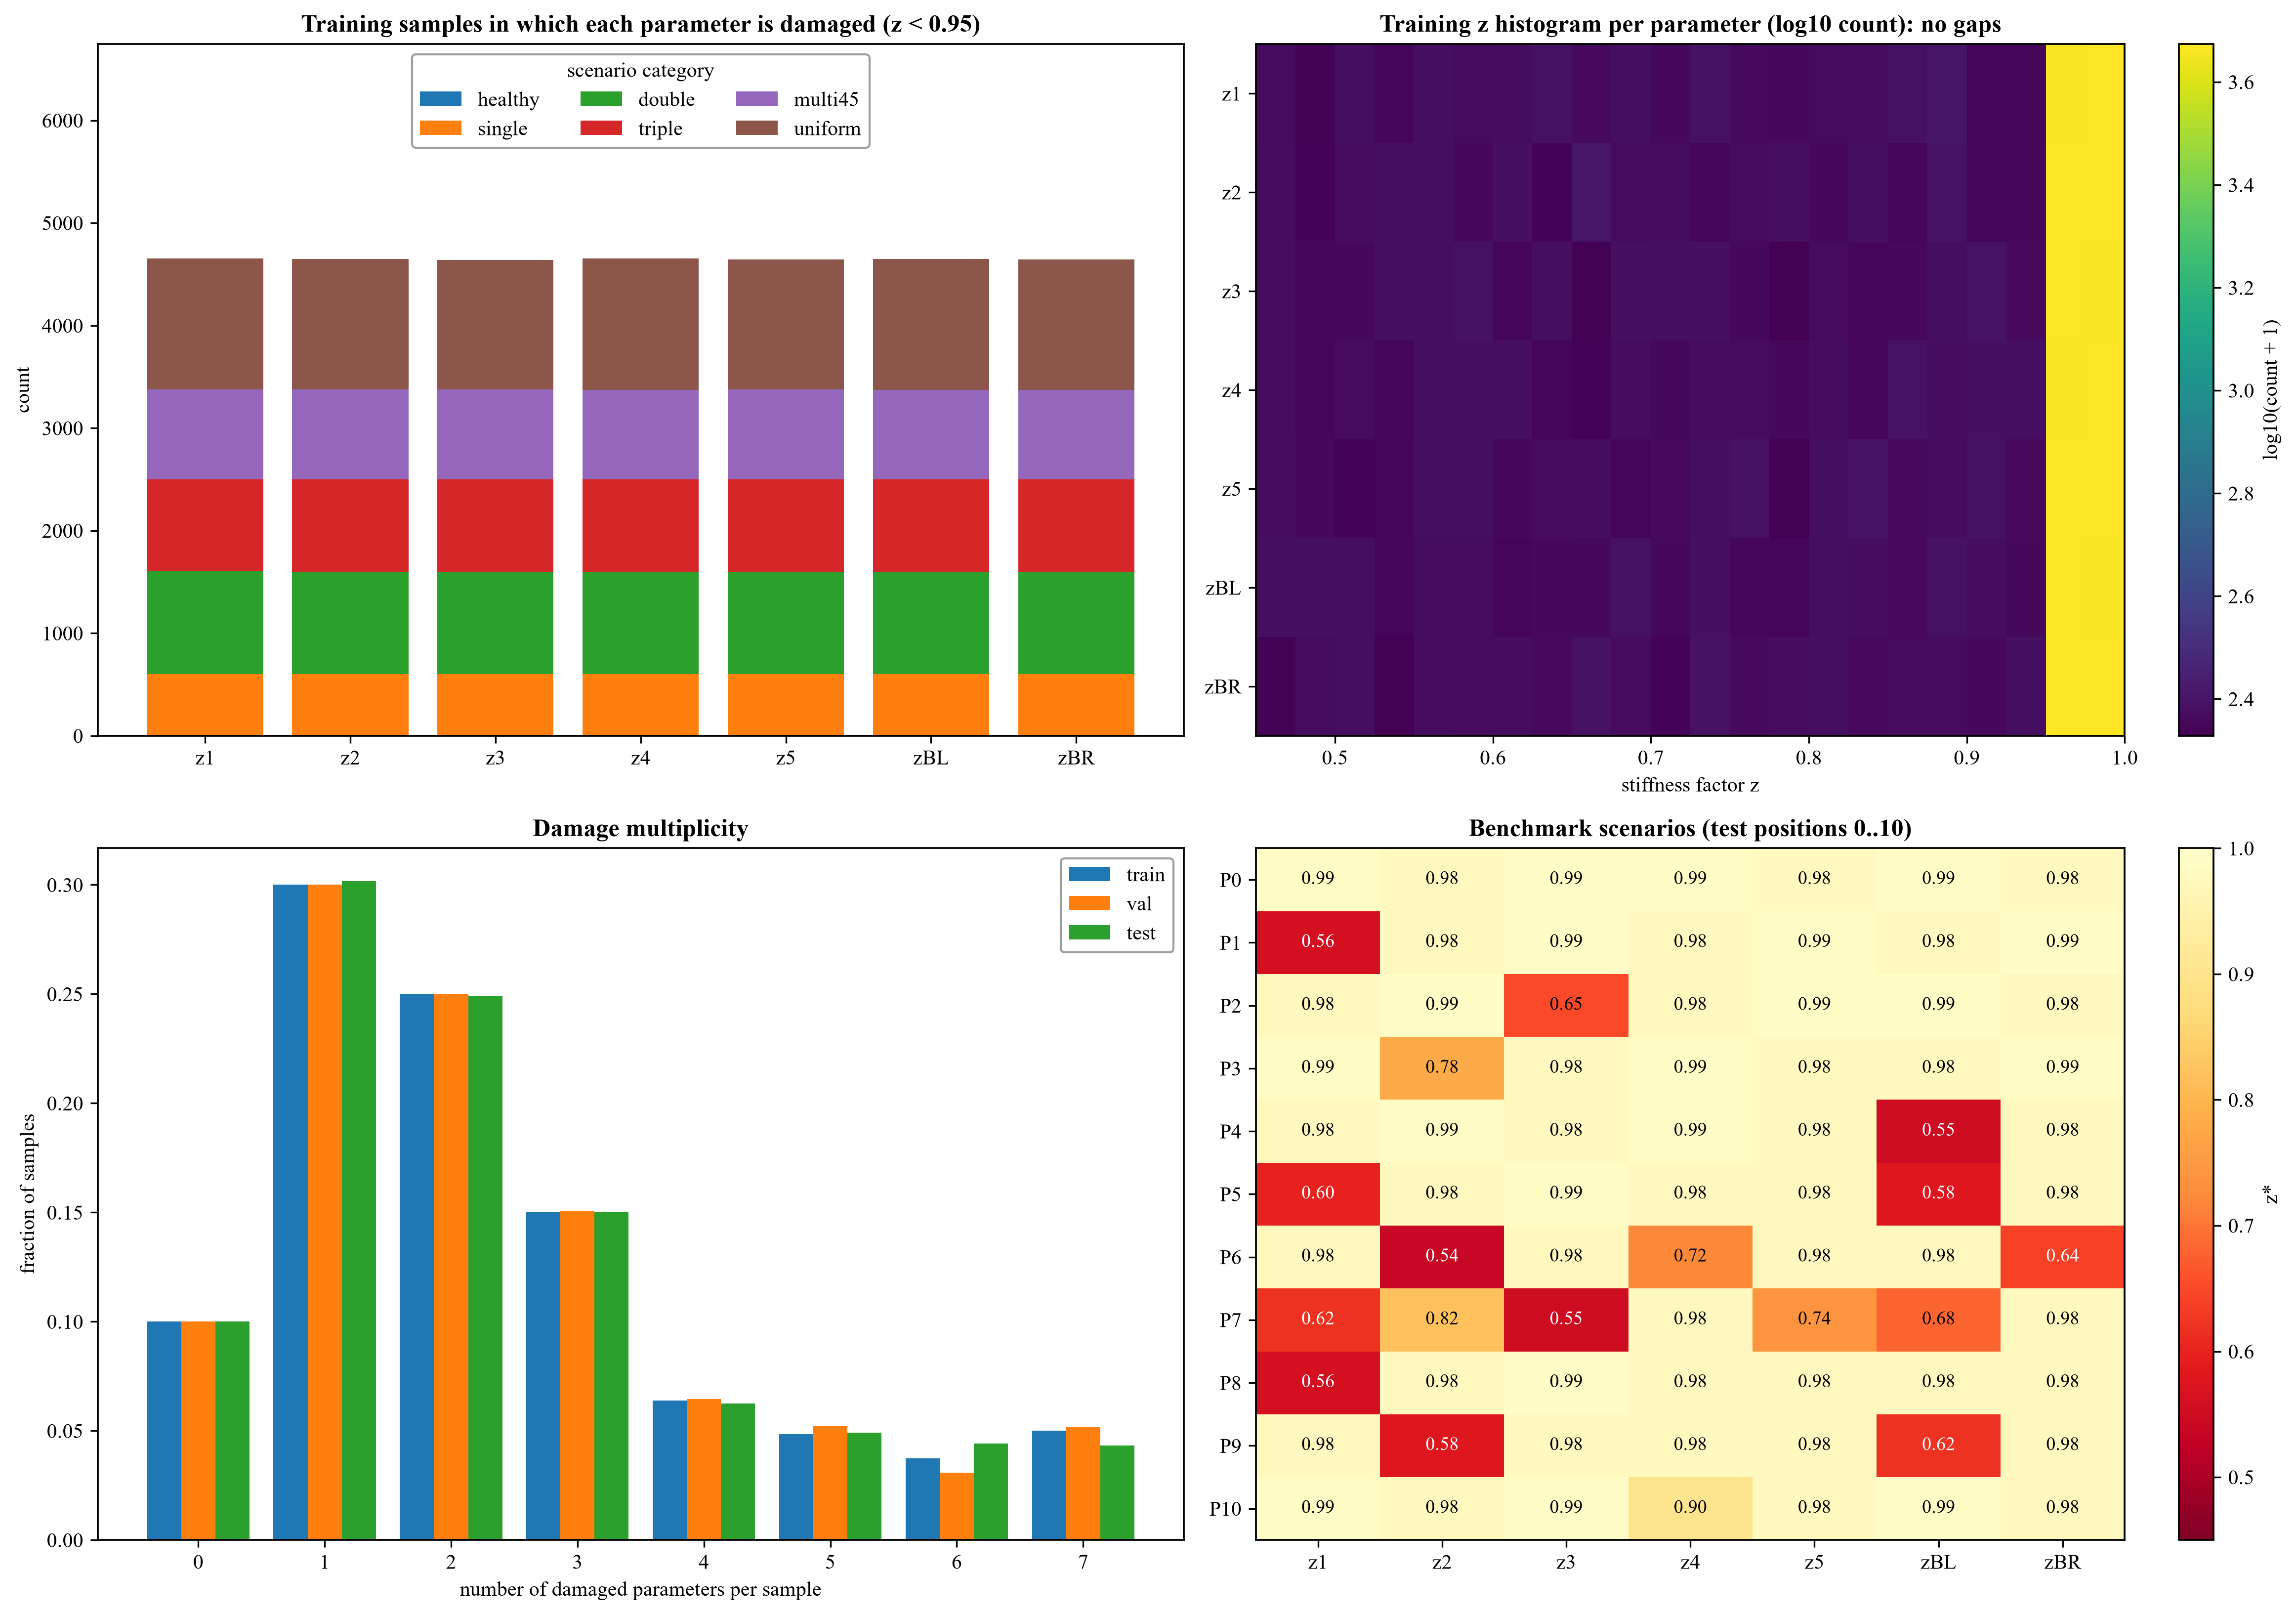
\includegraphics[width=0.95\textwidth]{figures_final/Fig_DoE_balance.png}
\caption{Design of experiments: number of training samples in which each parameter is damaged, per category;
histogram of the stiffness reduction factors; number of damaged parameters per sample in the training, validation and
test sets; and the eleven benchmark scenarios.}
\label{fig:doe}
\end{figure}

\begin{action}
New description of the DoE \lines{xx--yy} with Table~\tbd{x} and Fig.~\tbd{x}; false-alarm and detection rates reported
in \lines{xx--yy}.
\end{action}

% -----------------------------------------------------------------------------
\begin{rcomment}{7}
How does the proposed approach perform when the system is discretized more finely? The conclusion (lines 399-403)
refers to scalability to large-scale infrastructure. Could the authors comment on the expected computational and
statistical scaling of the method for systems with hundreds of elements, particularly given that the number of copula
correlation parameters and the computational cost of the eigensolver may both increase with problem size?
\end{rcomment}

\begin{response}
In the revised formulation, the FE discretization is decoupled from the damage parametrization. The latent variables
are the stiffness factors of the damage zones and bearings, and each zone may contain any number of elements
(Eq.~\eqref{eq:Kz}). The copula has $d(d-1)/2$ correlation parameters for $d$ latent variables (21 for $d=7$), a number
that depends on the number of damage zones and not on the number of elements. In the revised study, the decoder uses 10
elements (22 DOFs) instead of 5 without changing the latent dimension, and the trained model is tested on data from a
50-element model (102 DOFs) with localized damage, see R1.1.

\tbd{Results of the VAE on test set B.}
\end{response}
\authornote{discussion of the computational and statistical scaling still to be written: (i) structured correlation
matrices (banded, low-rank plus diagonal) keep the number of copula parameters linear in $d$; (ii) the decoder solves
one symmetric eigenproblem of size $n_{\mathrm{dof}}$ per sample, $O(n_{\mathrm{dof}}^3)$, batched; reduced-order
models or iterative solvers for the first $n_m$ modes would reduce this cost for hundreds of elements; (iii) report the
measured time per epoch for different meshes (currently about 2~s per epoch with the 22-DOF decoder and 1\,536
eigenproblems per step, solved on the CPU in double precision).}

\begin{action}
New paragraph on the decoupling of the mesh and the latent space \lines{xx--yy}. \tbd{scaling discussion.}
\end{action}

% -----------------------------------------------------------------------------
\begin{rcomment}{8}
A few references may benefit from a final consistency check. In particular, Reference 77 appears to contain placeholder
fields, and some references seem to be duplicated.
\end{rcomment}
\pending
\authornote{issues found in the submitted manuscript: Ref.~77 (Ding et al., 2026) has placeholder fields (author
``J.~Author'', journal ``Journal Name'', vol.~XX, pp.~XX--XX); Refs.~18 and 27 are the same paper (Simoen et al., 2015);
Refs.~56 and 57 are two editions of Przemieniecki's book; Kingma and Welling (2013) and Mottershead (1993) are listed but
not cited. The references must also follow the author--date style required by ASCE.}

% =============================================================================
\section{Reviewer \#2}
% =============================================================================

\begin{rcomment}{}
The paper presents a method based on physics-informed Gaussian copula variational autoencoder (PI-GCVAE) for
structural health monitoring (SHM) of simply supported bridges. The novelty lies in embedding a differentiable numerical
eigenvalue solver directly into the VAE architecture. The method is then demonstrated on a numerical study. The current
study is on a topic of relevance and general interest to the readers of the journal. However, I think the paper needs to
address several significant concerns and in my opinion has not yet reached the maturity to be published in CPENG
journal.
\end{rcomment}

\begin{response}
We thank the reviewer for the assessment. The concerns about the structural model motivated the main changes of the
revised case study: a girder line of a short-span composite bridge with realistic dimensions, elastomeric bearings, a
damage parametrization that includes the supports, two FE models (the second with localized damage), and modelling
errors in all the data. We describe them below.
\end{response}

% -----------------------------------------------------------------------------
\begin{rcomment}{1}
Introduction. The introduction is written well, but too much effort has been put on proving the methodological
novelty. I recommend focusing also on the utility to justify the value of the method for real bridges, as it seems that
the generalization of the approach is very difficult to other types of bridges considering the limitations of simply
supported bridge formulation and damage parametrization approach.
\end{rcomment}
\pending
\authornote{points for the revised introduction: the case study is now a realistic girder line on elastomeric bearings
whose damage is identifiable (R2.2); the formulation applies to any linear FE model whose stiffness is a weighted sum of
parameter matrices, so continuous bridges (intermediate bearings or piers) or other damage zones only add parameters;
the value for owners is a calibrated probability of damage per zone and bearing, which supports inspection
decisions.}

% -----------------------------------------------------------------------------
\begin{rcomment}{2}
Methodology. The assumption of simply-supported beam for single span bridges is not realistic. The majority of them
sits on elastic bearings whose effects are demonstrated in the literature. The formulation should at least include the
vertical springs at the ends.
\end{rcomment}

\begin{response}
We agree. The revised model replaces the simple supports by elastic bearings at both ends, each represented by a
vertical spring $k_v$ and a rotational spring $k_r$ (Fig.~\ref{fig:bridge}); since no degree of freedom is removed, the
model has $2(n_{\mathrm{el}}+1)$ DOFs. We also made the structure itself realistic. It is now a girder line of a
single-span steel--concrete composite bridge (Table~\ref{tab:specs}): an HEB~600 girder with a $2.0\times0.22$~m C30/37
slab, $EI=1.10\times10^{9}$~N\,m$^2$ and 1\,800~kg/m including the surfacing. Its first frequency, 11.9~Hz, lies within
the range given by EN~1991-2 for a 10~m span (8.0--16.9~Hz). The bearings are laminated elastomeric pads designed for the
reactions of this girder (88~kN under permanent loads): $200\times300$~mm in plan, three 8~mm rubber layers, shear
modulus $G=0.9$~MPa and shape factor $S=7.5$. The compression and rotation moduli of the pad, $6GS^2$ and $2GS^2$
corrected for the compressibility of the rubber (bulk modulus 2\,000~MPa), give $k_{v0}=6.6\times10^{8}$~N/m and
$k_{r0}=8.0\times10^{5}$~N\,m/rad. Each bearing has its own stiffness reduction factor, which scales both of its springs,
so that damage can occur in the deck and in the supports (Eq.~\eqref{eq:Kz}); the latent space has seven variables.
Since the comment concerns single-span bridges, the springs are placed at the two ends; the intermediate supports of a
continuous bridge would only add bearing parameters to Eq.~\eqref{eq:Kz}.

\textit{Why the deck had to change as well.} Adding springs to the beam of the submitted version would not have made the
model more realistic. That beam ($I=8.33\times10^{-6}$~m$^4$, 39~kg/m) was an academic section rather than a bridge
deck (Table~\ref{tab:old_new}):
\begin{itemize}[leftmargin=*]
\item its first frequency, 3.3~Hz, lies far below the range that EN~1991-2 gives for real bridges of a 10~m span
($80/L=8.0$ to $94.76\,L^{-0.748}=16.9$~Hz);
\item it deflects 28.7~mm ($L/350$) under its own weight only, whereas a bridge deck of this span deflects a few
millimetres under permanent loads;
\item its mass is 2\% of that of a real girder line, so the inertia, and thus the frequencies, were not representative.
\end{itemize}
With such a flexible deck, any realistic bearing is effectively rigid. A laminated pad sized for the small reactions of
that beam is still 430 times stiffer than the deck ($k_{v0}=3.6\times10^{7}$~N/m against $48EI/L^3=8.4\times10^{4}$~N/m):
it compresses 0.05~mm under the permanent load, while the deck deflects 28.7~mm at mid-span. The vertical springs would
store only 0.2--5.5\% of the modal strain energy, and a 55\% loss of stiffness of one bearing would change the
frequencies by 0.7--1.9\%, below the identification noise (2.5\%). The bearing parameters would then be practically
unidentifiable, not because bearings are invisible to vibration data, but because the deck was unrealistically
flexible. We therefore replaced the beam by the girder line of a real deck, designed the bearings for its reactions, and
checked that the result has the frequencies, deflections, and support stiffness of a short-span bridge.

\begin{table}[H]
\centering\small
\caption{Beam of the submitted version (with pads sized for its reactions) and girder line of the revised case study.
$k_{v0}$: vertical stiffness of one bearing; $48EI/L^3$: mid-span bending stiffness of the deck. Energy and frequency
changes for modes 1--5; frequency change for a 55\% loss of stiffness of one bearing ($z_{b,L}=0.45$).}
\label{tab:old_new}
\footnotesize
\begin{tabular}{p{5.0cm}p{4.6cm}p{5.0cm}}
\toprule
 & Submitted version (+ elastic pads) & Revised case study \\
\midrule
Cross-section & academic section, $I=8.33\times10^{-6}$~m$^4$ & HEB~600 + $2.0\times0.22$~m C30/37 slab,
$I=5.25\times10^{-3}$~m$^4$ (steel units) \\
Bending stiffness $EI$ & $1.75\times10^{6}$~N\,m$^2$ & $1.10\times10^{9}$~N\,m$^2$ \\
Mass per unit length & 39~kg/m (steel only) & 1\,800~kg/m (girder, slab, surfacing, edges) \\
First frequency (EN~1991-2 range: 8.0--16.9~Hz) & 3.3~Hz (outside) & 11.9~Hz (inside) \\
Mid-span deflection, permanent load & 28.7~mm ($L/350$) & 2.1~mm ($L/4\,800$) \\
Bearing (laminated pad) & $S=3$, $k_{v0}=3.6\times10^{7}$~N/m & $200\times300$~mm, $S=7.5$, $k_{v0}=6.6\times10^{8}$~N/m \\
Pad compression, permanent load & 0.05~mm & 0.13~mm \\
$k_{v0}/(48EI/L^3)$ & 430 (bearings effectively rigid) & 12.5 \\
Energy in the vertical springs & 0.2--5.5\% & 6.4--55.4\% \\
Frequency change, $z_{b,L}=0.45$ & $-0.7$ to $-1.9$\% (below the noise) & $-2.0$ to $-12.3$\% \\
\bottomrule
\end{tabular}
\end{table}

\textit{Effect of the bearings.} The sensitivity of the squared frequency of a mode to the stiffness of a spring equals
the fraction of the modal strain energy stored in that spring. With realistic proportions, the vertical flexibility of
the pads is not negligible compared with the bending flexibility of the deck ($k_{v0}$ is only 12.5 times larger than
$48EI/L^3$): the vertical springs store 6--56\% of the strain energy of the five modes (Table~\ref{tab:bearing_energy}),
and the bearings lower the first frequency from 12.29~Hz (simple supports) to 11.91~Hz. The pads are designed to let the
girder rotate ($k_{r0}L/EI=0.007$), so the rotational springs store less than 0.3\% of the energy. Consequently, a 55\%
loss of stiffness of one bearing changes the frequencies by 2.0--12.3\% and the mode shapes by up to 0.10 in
$1-\mathrm{MAC}$, well above the identification noise (2.5\% and about $4\times10^{-3}$), and bearing degradation is
identifiable from the vertical modes of the deck. For instance, the exact posterior of benchmark P4 (left bearing,
$z_{b,L}=0.55$) has mean 0.52 and standard deviation 0.03, against 0.16 for the prior, with no false alarm in the deck
(Fig.~\ref{fig:bearing}). The bearing factor is identified through the vertical stiffness of the pad; the rotational
stiffness has a negligible effect, as intended in the design of elastomeric bearings.

\textit{Summary of the modelling assumptions.} (i) Euler--Bernoulli beam ($L/h\approx12$ with the slab). Shear deformation and rotary inertia are small for the
first modes and would lower the highest frequencies by a few percent (mode 5 has half-waves of 2~m); since the same
beam theory produces the data and the decoder, this does not affect the conclusions of the numerical study, and with
field data it would be part of the model discrepancy of R1.2. (ii) Full composite action between girder and slab (shear connectors), with the slab transformed with the
modular ratio $n=E_s/E_c=210/33$. (iii) One girder line: the vertical bending modes of a deck with several girders and
a transverse distribution of the loads are represented by the stiffness and mass of one girder and its tributary slab.
(iv) Linear, elastic bearings with vertical and rotational stiffness from the standard expressions for laminated pads;
the longitudinal (shear) stiffness of the pads does not enter the vertical bending modes and is not modelled.
(v) Damage is a loss of bending stiffness of a deck zone or a loss of vertical (and rotational) stiffness of a bearing.
(vi) Modelling errors in the mass and in the stiffness inside each zone are included in all the data (R1.2). Which types
of damage can and cannot be detected with this model is discussed in R2.3.
\authornote{add references for the design of elastomeric bearings (EN~1337-3; AASHTO LRFD Section 14), for the effect
of bearings on bridge dynamics, and EN~1991-2 for the frequency range. Table~\ref{tab:old_new}: confirm that the beam
of the submitted version had $I=8.33\times10^{-6}$~m$^4$ and $A=0.005$~m$^2$ (values of the code in
MODULES/review29oct); the ``+ elastic pads'' column is the intermediate model with pads sized for that beam
($S=3$, $k_{r0}=6.8\times10^{4}$~N\,m/rad). Numbers recomputed with a 50-element Euler--Bernoulli model.}
\end{response}

\begin{table}[H]
\centering\small
\caption{Share of the modal strain energy stored in the bearings of the healthy bridge, and change of the natural
frequencies and mode shapes when one bearing loses 55\% of its stiffness ($z_{b,L}=0.45$).}
\label{tab:bearing_energy}
\begin{tabular}{lccccc}
\toprule
 & Mode 1 & Mode 2 & Mode 3 & Mode 4 & Mode 5 \\
\midrule
Energy in the vertical springs (\%) & 6.4 & 25.7 & 52.1 & 55.8 & 32.9 \\
Energy in the rotational springs (\%) & 0.27 & 0.04 & $<0.01$ & 0.01 & 0.02 \\
Frequency change, $z_{b,L}=0.45$ (\%) & $-2.0$ & $-7.8$ & $-12.3$ & $-8.5$ & $-4.2$ \\
$1-\mathrm{MAC}$ of the vertical shapes, $z_{b,L}=0.45$ & 0.001 & 0.026 & 0.072 & 0.102 & 0.061 \\
\midrule
Identification noise of the frequencies (\%) & 2.5 & 2.5 & 2.5 & 2.5 & 2.5 \\
\bottomrule
\end{tabular}
\end{table}

\begin{figure}[H]
\centering
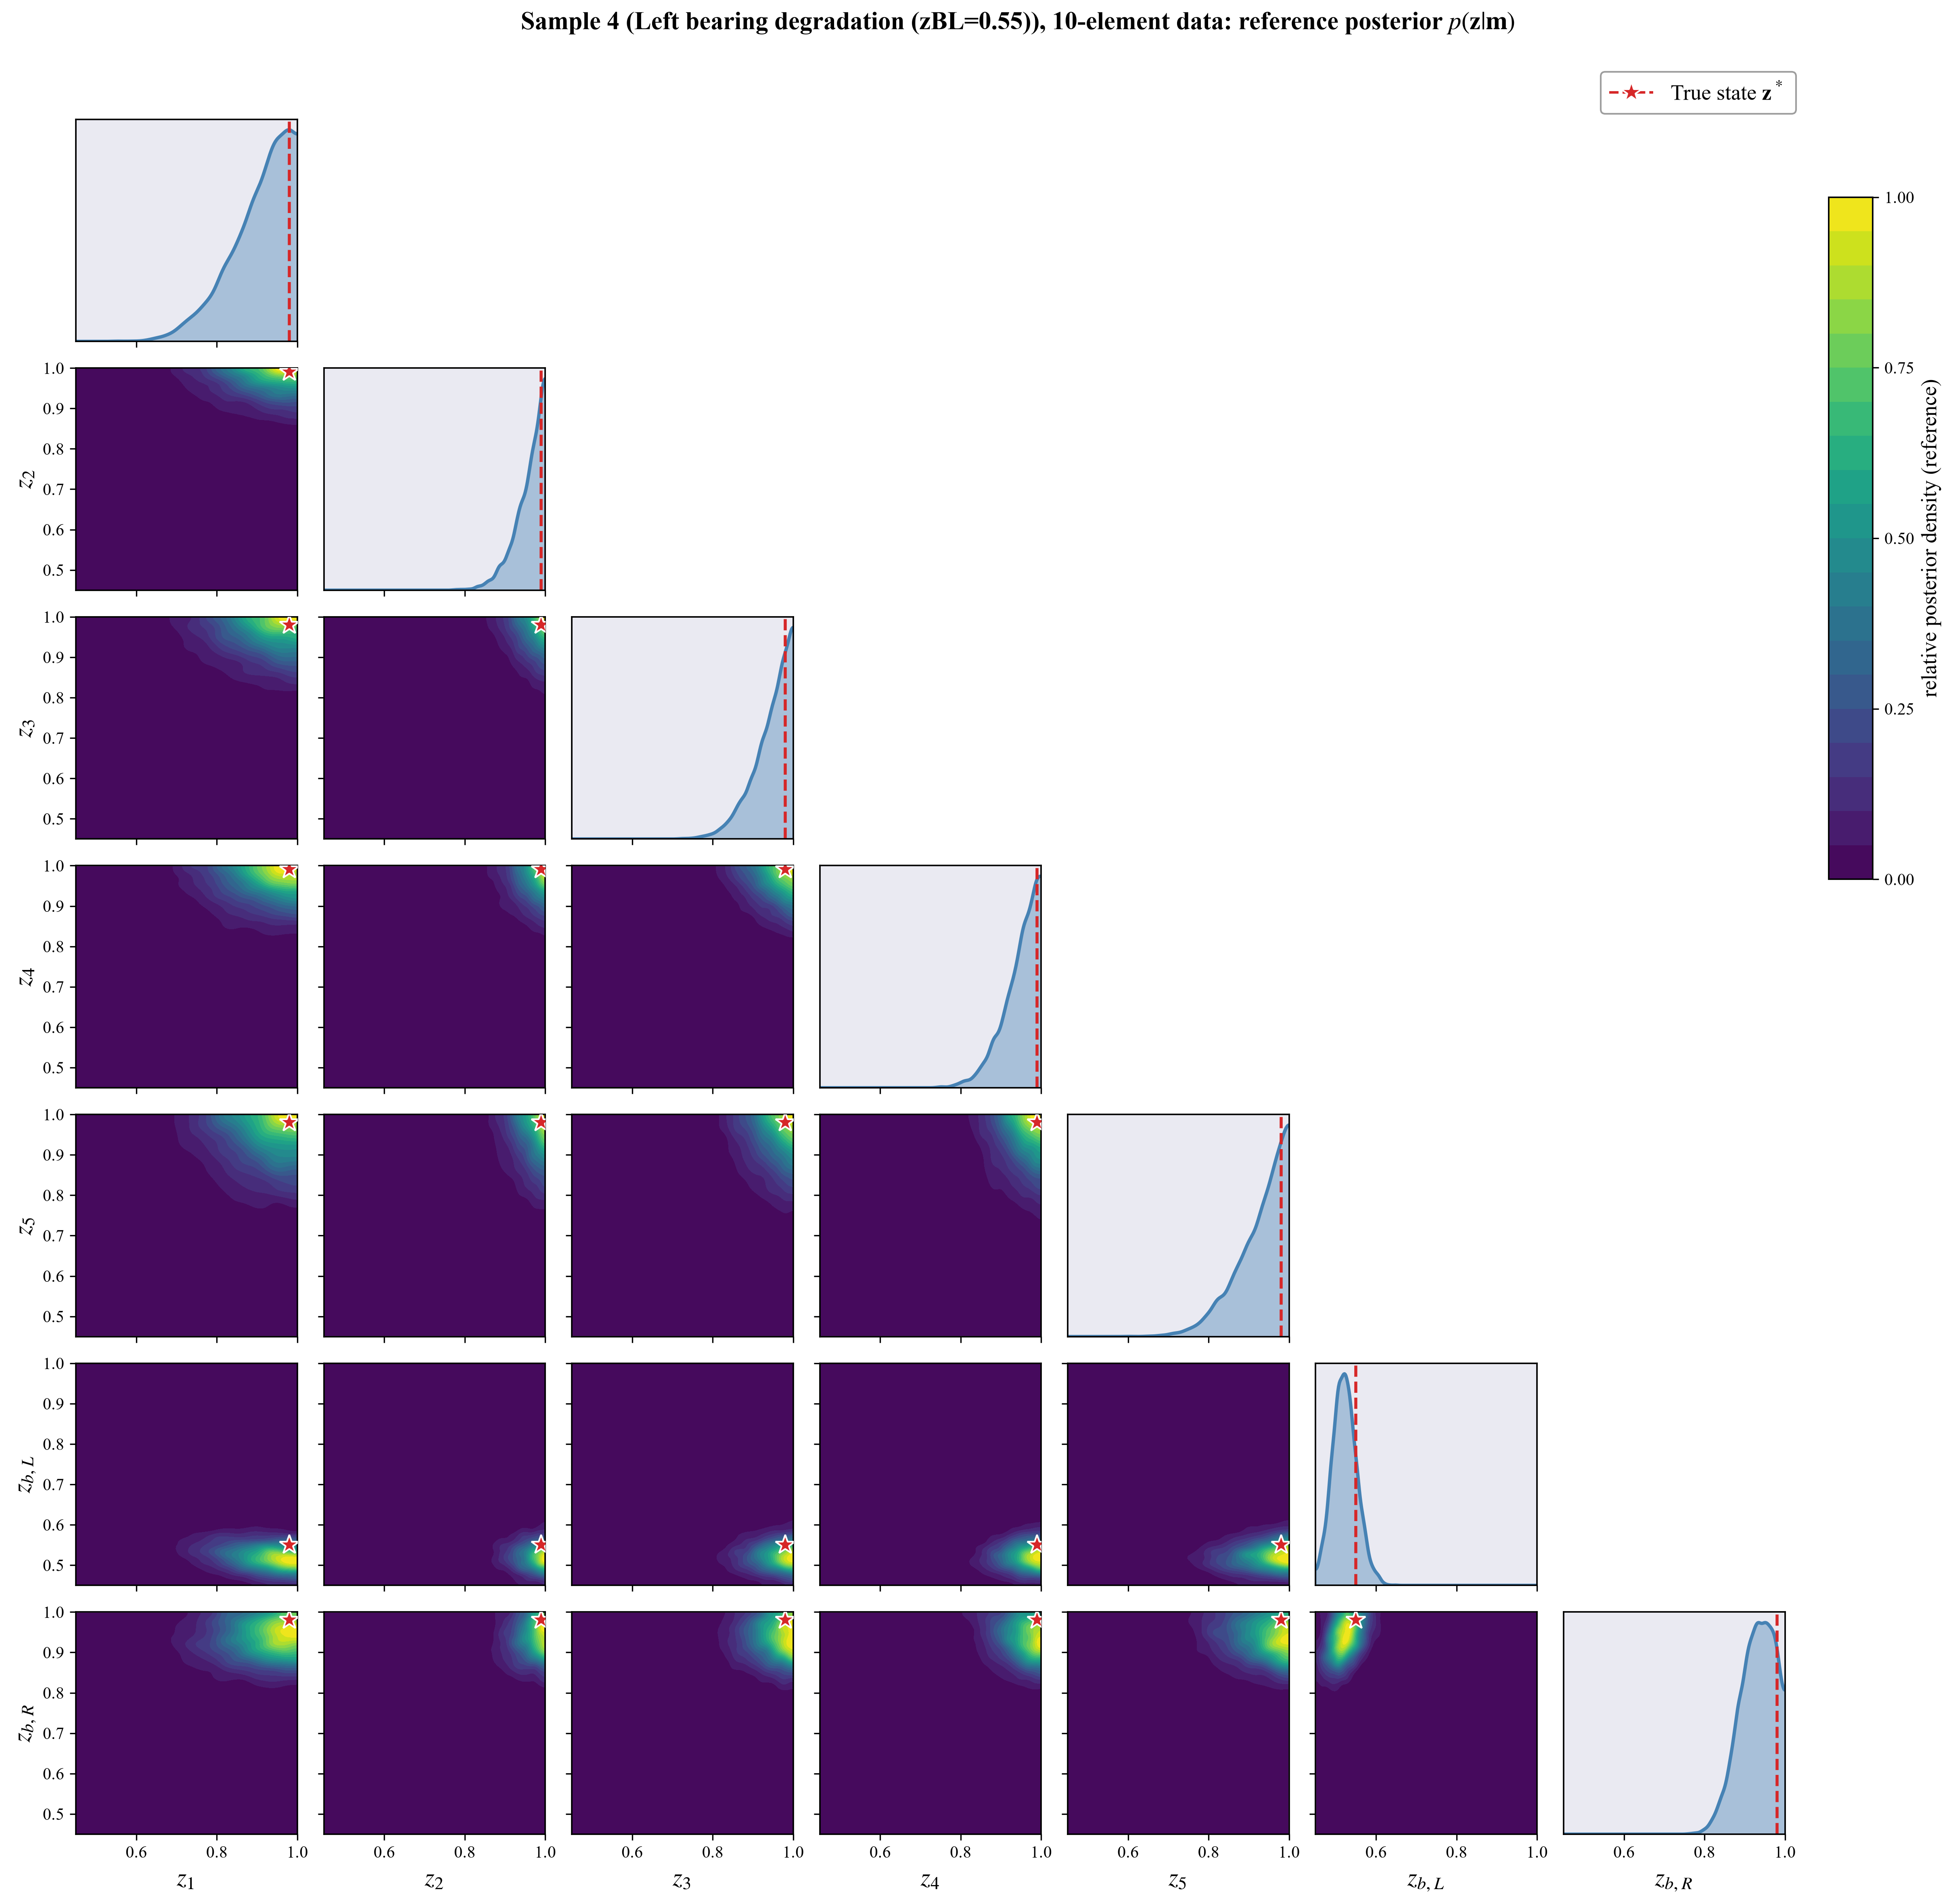
\includegraphics[width=0.62\textwidth]{figures_final/Fig_reference_posterior_P4_test.png}
\caption{Exact posterior of benchmark P4 (left bearing degraded, $z_{b,L}=0.55$; test set A). The red stars mark the true
damage condition.}
\label{fig:bearing}
\end{figure}

\begin{action}
New FE model of a girder line of a composite bridge on elastomeric bearings, with seven unknowns \lines{xx--yy},
Fig.~\tbd{x} (Fig.~\ref{fig:bridge}) and Tables~\tbd{x} (Tables~\ref{tab:specs} and~\ref{tab:bearing_energy}).
\end{action}

% -----------------------------------------------------------------------------
\begin{rcomment}{3}
Methodology. Another limitation is the damage parametrization presented as a ``local'' loss of stiffness distributed
within an element of a specific length. Considering the type of the bridge, this type of damage parametrization is not
realistic, neither for steel bridges nor for RC. This point seems particularly important as the novelty of the proposed
methodology is presented as capturing the interconnectedness of damage scenarios. I recommend, in line with the comment
above, including the support conditions in the formulation, which can enable to detect damage observed there.
\end{rcomment}

\begin{response}
We have revised the parametrization in three ways.

\textit{Support conditions.} As recommended, the stiffness of each bearing is now an unknown of the problem
($z_{b,L}$, $z_{b,R}$), so the formulation represents damage at the supports. Three benchmark scenarios include bearing
degradation (P4, P5 and P9), and the training data contain bearing damage alone and combined with deck damage. With
realistic proportions, the bearings are identifiable (R2.2): in the exact posteriors of the benchmarks, the standard
deviation of the bearing factors is 0.02--0.05, against 0.16 for the prior. Damage at a support and damage of the
adjacent end zone can partly compensate each other, and the copula represents this dependence (P5,
Fig.~\ref{fig:testfine}). Bearing defects that increase the stiffness (hardening of the elastomer, seized bearings) lie
outside the support of the prior; their effect is examined in R1.5.

\textit{Which damage the vertical bending modes can detect.} The features used in this study are the frequencies and
vertical mode shapes of the bending modes of the deck. They are global quantities, and the sensitivity of each one to a
parameter is proportional to the fraction of the modal strain energy stored in the corresponding element. They are
therefore suited to damage that reduces the \emph{vertical bending stiffness} of the deck: flexural cracking of the
concrete slab after overloading or fatigue, loss of section by corrosion of the reinforcement or of the steel girder,
fatigue cracks in the flanges, impact of vehicles on the girder, fire, and flexural damage of the deck after an
earthquake. At the supports, they detect the loss of \emph{vertical} stiffness of the bearings.

In the revised case study, the bearings are among the best identified parameters. In benchmark P4 ($z_{b,L}=0.55$),
the posterior of the VAE concentrates between about 0.47 and 0.60 and agrees with the exact posterior, while the deck
zones remain at their healthy values. There are three reasons:
\begin{enumerate}[leftmargin=*]
\item \emph{A bearing affects every mode.} The supports move in all five modes (6--56\% of the strain energy,
Table~\ref{tab:bearing_energy}), so all frequencies and mode shapes carry information about each bearing. A 2~m deck
zone mainly affects the modes with large curvature in that zone; the end zones, where the curvature of the low modes is
small, are the least identified deck parameters.
\item \emph{The sensitivity increases with the damage.} The pad acts in series with the deck, and its flexibility is
proportional to $1/z_b$. A degraded bearing therefore changes the modal data more per unit of $z_b$ than a healthy one,
and its posterior is narrower: healthy bearings are identified within about 0.8--1.0, and a bearing with $z_b=0.55$
within about $\pm0.06$.
\item \emph{Few compensating parameters.} A deck zone can be partly compensated by both neighbours, while a bearing can
only be partly compensated by the adjacent end zone. When both are damaged, the posterior of the bearing widens and
becomes correlated with that of the end zone (P5, Fig.~\ref{fig:testfine}), and the copula represents this dependence.
\end{enumerate}

This identifiability is a property of short, stiff spans, and we state its limits explicitly in the revised manuscript:
\begin{itemize}[leftmargin=*]
\item \emph{Span.} The ratio between the stiffness of the pad and the bending stiffness of the deck, $k_{v0}/(48EI/L^3)$,
grows with $L^3$. With the same section and pads, it is 12.5 for $L=10$~m, 100 for 20~m and 340 for 30~m; the share of
the strain energy in the springs drops to 0.8--26\% and 0.2--7\%, and a 55\% loss of stiffness of one bearing changes
the frequencies by at most 7.6\% and 2.3\%, respectively. For longer spans, the bearings become almost rigid for the
vertical modes, as for the beam of the submitted version (Table~\ref{tab:old_new}).
\item \emph{Damage mechanisms of real bearings.} The most frequent defects of elastomeric and sliding bearings, such as
hardening of the elastomer with age and low temperature, cracking or delamination of the rubber layers, slipping or
walking of the pad, and seized sliding or guided bearings, mainly change the \emph{shear (longitudinal)} stiffness and the
rotational behaviour of the bearing, and hardly change its vertical stiffness. The longitudinal stiffness does not enter
the vertical bending modes, and the rotational springs store less than 0.3\% of their energy, so these defects are not
observable with the features of this study. Defects that stiffen the bearing lie outside the prior; their effect is
examined in R1.5.
\end{itemize}
These defects require measurements of the longitudinal response at the bearings. In a previous study
(Garcia-Sanchez et al., 2020), we assessed the bearings of a prestressed concrete viaduct from long-term measurements of
the longitudinal displacements at the bearings, with an unsupervised, temperature-insensitive indicator based on
principal component analysis. The two approaches are complementary: local longitudinal measurements to assess the
condition of the bearings, and global vertical modal data to identify, locate and quantify losses of bending stiffness
of the deck and of vertical stiffness of the supports, with a calibrated uncertainty.
\tbd{VAE results for the bearings: posterior standard deviations and coverage of $z_{b,L}$, $z_{b,R}$ vs.\ deck zones;
detection rate of bearing damage vs.\ severity; benchmarks P4, P5 and P9.}

\textit{Zone-wise damage parameters.} The deck parameters are no longer the stiffness of individual elements but the
equivalent bending stiffness of 2~m damage zones, which is independent of the mesh (two elements per zone in the
decoder, ten in the 50-element model). This is the spatial resolution that five accelerometers and five modes can
provide (R3.4). In reinforced-concrete decks, flexural cracking spreads over a region of the span, and the reduction of
the equivalent stiffness of that region is the usual representation in vibration-based model updating (e.g., Teughels
et al., 2002); in steel girders, a loss of section by corrosion, frequent near the supports, or a local defect reduce
the equivalent stiffness of the zone that contains them.

\textit{Localized damage inside the zones.} To test this representation when the actual damage is localized, the second
test set concentrates the loss of stiffness of every damaged zone in a sub-region of 0.2--2.0~m at a random position,
with the same equivalent stiffness (R1.1); the stiffness of the damaged sub-region drops to 15--95\% of its nominal value.
The decoder only knows the zone-wise parametrization, so this is a genuine model-form error, of the same size as that of
the mass deviations (Table~\ref{tab:budget}). The exact posteriors from this test set still contain the true equivalent
stiffness for 69 of the 77 parameters of the benchmarks. In addition, R1.5 tests short defects that are not aligned with
the zones, including defects next to the supports.
\tbd{VAE results on test set B and on the defects of R1.5.}
\authornote{(i) add the reference: D.~Garcia-Sanchez, A.~Fernandez-Navamuel, D.~Zamora S\'anchez, D.~Alvear and
D.~Pardo (2020), Bearing assessment tool for longitudinal bridge performance, J.\ Civil Struct.\ Health Monit.\ 10(5),
1023--1036, doi:10.1007/s13349-020-00432-1, and references for the damage mechanisms of bearings (e.g., NCHRP reports on
bearing condition, EN~1337-3). (ii) The P4 interval (0.47--0.60) and the healthy range (0.8--1.0) are read from the
violin plots of the 3KS run (TestA, Sample\_0 and Sample\_4); replace them with the exact values of the final tables.
(iii) The span study uses the same section for 20 and 30~m (illustrative: a longer span would have a deeper section,
but $EI/L^3$ still decreases). (iv) Add the same discussion of scope to the manuscript (case study and conclusions).}

\textit{Interconnectedness of damage scenarios.} The correlations captured by the copula reflect how the modal data
constrain combinations of parameters: adjacent zones are negatively correlated because a softer zone can be partly
compensated by a stiffer neighbour, and the same holds for an end zone and the adjacent bearing.
\end{response}

\begin{action}
New parametrization with bearing factors and zone-wise stiffness factors \lines{xx--yy}; localized damage in the
second test set \lines{xx--yy}; discussion of the parametrization for concrete and steel decks \lines{xx--yy}.
\end{action}

% -----------------------------------------------------------------------------
\begin{rcomment}{4}
Methodology. The numerical case study, 5-elements simply supported beam is too simplistic. I would recommend at least
considering a more realistic case and testing the proposed method on a lab scale beam.
\end{rcomment}

\begin{response}
We agree that the original case study was too simple. The revised case study (Fig.~\ref{fig:bridge},
Table~\ref{tab:specs}) is a girder line of a short-span composite bridge with realistic dimensions, mass and
frequencies, on elastomeric bearings designed for its reactions, with seven unknowns (five deck zones and two bearings).
It uses a 10-element decoder model, modelling errors (mass and stiffness deviations) in all the data, a second test set
from a 50-element model with localized damage, six additional test sets outside the training distribution (R1.5), a
realistic sensor layout with five accelerometers, and the first five bending modes identified with realistic noise.
The structure was checked against the properties of real short-span bridges: first frequency within the range of
EN~1991-2, deflection and pad compression under permanent loads, and bearing stress under traffic loads
(Table~\ref{tab:old_new} and R2.2). R2.3 discusses which types of damage this model can and cannot identify.
\end{response}
\authornote{validation on a laboratory-scale beam still pending; otherwise, discuss it as a limitation and future
work.}

\begin{action}
New case study \lines{xx--yy}.
\end{action}

% =============================================================================
\section{Reviewer \#3}
% =============================================================================

\begin{rcomment}{}
In this manuscript, a novel probabilistic machine learning framework is presented for vibration-based damage
identification in civil infrastructure. The SHM approach employs a physics-informed Gaussian copula variational
autoencoder. The effectiveness of the framework is explored in detail and validated under various damage scenarios
using synthetic, noise-contaminated data of a simply supported bridge. The manuscript contains novel theoretical
developments that are worth publishing. Before publication, the following issues have to be addressed.
\end{rcomment}

\begin{response}
We thank the reviewer for the positive evaluation and for the detailed comments, which we address below.
\end{response}

% -----------------------------------------------------------------------------
\begin{rcomment}{1}
In Bayesian finite element model updating, the discrepancy between the physical structure and the parameterized
mathematical model (i.e., modeling error) dominates over sensor noise. The current validation assumes a perfectly known
baseline mass matrix and attributes all dynamic discrepancies to stiffness reductions (which are updated in the process)
and artificial Gaussian noise. To demonstrate the robustness of the PI-GCVAE, the authors must explore its sensitivity
to modeling errors (e.g., small random perturbations to the mass matrix) and investigate how such unmodeled dynamics
propagate into the posterior uncertainty bounds for the stiffness reduction factors.
\end{rcomment}

\begin{response}
We agree, and we followed the reviewer's suggestion. In the revised study, the baseline mass matrix is no longer
perfectly known. Every measurement, in the training, validation and test sets, comes from an as-built structure whose
mass differs from the nominal mass used by the decoder: the mass of each 1 m segment is multiplied by $1+\mu_s$, with
$\mu_s\sim\mathcal{N}(0,0.05^2)$ (Eq.~\eqref{eq:asbuilt}). The data also include stiffness variations inside the
damage zones and, in the second test set, a finer discretization and localized damage (R1.2). The decoder keeps the
nominal mass matrix, and
the realizations of these perturbations are never available to the VAE.

\textit{Propagation into the posterior.} These unmodelled effects enter the inference through the likelihood
(Eqs.~\eqref{eq:discrepancy} and~\eqref{eq:nll}). We estimate their effect on the observations by simulation: the mass
perturbations alone change the frequencies with a standard deviation of 0.91--1.09\% and the mode shapes by up to
$3.3\times10^{-3}$ in $1-\mathrm{MAC}$ (Table~\ref{tab:budget}, Fig.~\ref{fig:budget}). Combined with the measurement
noise, the standard deviation of the log-frequency errors increases from 2.5\% to 2.66--2.72\%, and that of the
mode-shape components from 0.027--0.033 to 0.028--0.044. Since these values define the likelihood, the posterior bounds of the stiffness
factors widen consistently with what the decoder cannot represent, instead of attributing the mass deviations to
stiffness changes with false confidence. The calibration check on independent data confirms that the likelihood
describes the actual deviations (Fig.~\ref{fig:calib}). With this setup, the exact posteriors of the benchmark scenarios
have standard deviations of 0.03--0.12 for the deck zones and 0.02--0.05 for the bearings. Two of the test sets of R1.5
examine what happens when the modelling error is larger than assumed (twice the mass and stiffness deviations) or
systematic (additional mass not included in the model).
\tbd{Posterior bounds and coverage of the VAE with modelling error; comparison with the exact posterior.}
\end{response}
\authornote{(i) The reviewer states that modelling error dominates over sensor noise; with 5\% mass deviations, the
modelling error ($\approx$1\% on the frequencies; 1.2--1.8\% in test set B, with the localized damage) is smaller than
the identification noise (2.5\%); discuss this together with the larger modelling errors of R1.5. (ii) A direct
quantification of the propagation would
strengthen the answer: exact posteriors and coverage with a likelihood that ignores the modelling error vs.\ the
calibrated likelihood, on the same data.}

\begin{action}
New subsection on modelling errors and their propagation \lines{xx--yy}; Table~\tbd{x} and Fig.~\tbd{x}.
\end{action}

% -----------------------------------------------------------------------------
\begin{rcomment}{2}
In the ``Sensitivity to $\gamma$ hyperparameter and model selection'' section, the hyperparameter $\gamma$, which
balances the data likelihood and the prior regularization, is calibrated based on the performance of the model on the
test dataset. This approach compromises the independence of the test set and results in overly optimistic performance
estimates. The optimal value of $\gamma$ must be selected using only the validation dataset. The authors need to
correct this methodological flaw and subsequently report the unbiased performance metrics on the completely unseen test
set.
\end{rcomment}

\begin{response}
We agree with the reviewer and thank them for identifying this flaw. In the revised formulation, $\gamma$ is no longer
a tuned hyperparameter. Since the data terms of the loss are now the calibrated negative log-likelihood
(Eq.~\eqref{eq:nll}), the loss of Eq.~\eqref{eq:loss} with $\gamma=1$ is the negative ELBO, whose minimizer is the
Bayesian posterior; values $\gamma\neq1$ would produce tempered posteriors without a probabilistic interpretation. We
therefore fix $\gamma=1$ a priori. The only choice made with data is the selection of the trained model: we keep the
weights with the lowest negative ELBO on the validation set, after a warm-up of 150 epochs in which the weight of the
likelihood grows from 0.01 to 1. The number of Kumaraswamy components is selected in the same way, with the
validation negative ELBO (R1.4). The test sets are used only once, to compute the reported metrics.
\tbd{Unbiased metrics on the test sets.}

\textit{Role of $\gamma$ and sensitivity analysis.} For $\gamma\neq1$, the minimizer of Eq.~\eqref{eq:loss} is the
variational approximation of the tempered posterior $p_\gamma(\z|\m)\propto\exp\big(-\mathrm{NLL}(\z;\m)/\gamma^2\big)\,
p(\z)$: $\gamma<1$ sharpens the posterior (overconfident intervals) and $\gamma>1$ widens it (conservative intervals).
In the revised formulation, the width of the posterior is therefore set by the statistics of the measurement and
modelling errors in the likelihood (R1.2, R1.3), not by $\gamma$. To show this, and to document how sensitive the
results are to this choice, we add a sensitivity analysis in which the model is retrained with
$\gamma\in\{0.5,0.75,1,1.5,2\}$ ($\gamma^2$ from 0.25 to 4), all other settings unchanged. For each value we report,
on the validation set only, the empirical coverage and the MACE of the credible intervals, the error of the posterior
mean, and the agreement with the exact posteriors computed with the same $\gamma$. We expect the posterior means to be
almost insensitive to $\gamma$ and the coverage to be closest to its nominal value at $\gamma=1$. This analysis
illustrates the effect of $\gamma$ and is not used to select it: $\gamma=1$ is kept for all the reported results.
\tbd{Results of the sensitivity analysis: coverage and MACE vs.\ $\gamma$ (figure), error of the posterior mean.}
\end{response}
\authornote{(i) Sensitivity study not run yet: 4 additional trainings ($\gamma=0.5$, 0.75, 1.5, 2). (ii) The submitted
version used $\gamma=0.30$ (R1.3) and the old code of October used $\gamma=0.35$; check which value the submitted manuscript
reports. (iii) Test set B is misspecified (localized damage, R1.1), and $\gamma$ slightly above 1 may calibrate better
there (power/generalized posteriors, e.g., Gr\"unwald and van Ommen, 2017). If we want to discuss this, we need a
validation set generated like test set B, so that the test sets are still not used for any choice.}

\begin{action}
Section ``Sensitivity to $\gamma$ hyperparameter and model selection'' rewritten \lines{xx--yy}.
\end{action}

% -----------------------------------------------------------------------------
\begin{rcomment}{3}
Within the Bayesian setting, the posterior is heavily dependent on the choice of the prior $p(\z)$. The formulation
assumes a bounded uniform prior $\mathcal{U}[0.5,1.0]$. At the same time, the synthetic training dataset is generated
by uniformly sampling the same space. In actual SHM applications, severe damage is highly improbable; thus, a realistic
prior should strongly penalize large reductions in stiffness. The authors should clarify the distinction between the
generative sampling density used for training (which might be uniform to prevent class imbalance) and the theoretical
Bayesian prior incorporated in the ELBO loss. Can the current framework accommodate an informative, non-uniform prior
while training on uniform data? A brief discussion on this decoupling is necessary.
\end{rcomment}

\begin{response}
We thank the reviewer for this important remark, which we now discuss explicitly. Two different distributions play a
role:
\begin{itemize}[leftmargin=*]
\item The \emph{prior} $p(\z)$ is part of the Bayesian model. It enters the loss through the negative ELBO of each
observation,
\begin{equation}
-\mathrm{ELBO}(\m)=\mathbb{E}_q\big[\mathrm{NLL}(\z;\m)\big]+\mathbb{E}_q\big[\log q(\z|\m)\big]
-\mathbb{E}_q\big[\log p(\z)\big],
\label{eq:elbo_prior}
\end{equation}
and through the reference posterior.
\item The \emph{sampling density} of the training data (the DoE) only determines which observations the encoder sees
during training. The loss is an average over observations of Eq.~\eqref{eq:elbo_prior}, and for each observation its
minimizer is the posterior $p(\z|\m)\propto p(\m|\z)\,p(\z)$, independently of how often that observation appears in the
training set. The DoE therefore determines where the amortized encoder is accurate, not which posterior it targets.
\end{itemize}
The revised study makes this decoupling explicit: the prior is uniform on $[0.45,1]^7$, whereas the DoE is a balanced
mixture of healthy and localized damage scenarios (R1.6) that is far from uniform (two thirds of the parameters lie in
$[0.95,1]$). For a uniform prior, the last term of Eq.~\eqref{eq:elbo_prior} is constant, which is why the loss only
contains the likelihood and the entropy. An informative prior, e.g., one that penalizes large stiffness reductions,
only requires adding $-\mathbb{E}_q[\log p(\z)]$ to the loss, estimated with the same samples of $q$, and using the same
prior in the reference posterior. Neither the training data nor the architecture change.
\end{response}
\authornote{optional: demonstrate an informative prior on one benchmark.}

\begin{action}
New paragraph on the prior and the sampling density of the training data \lines{xx--yy}, with
Eq.~\eqref{eq:elbo_prior}.
\end{action}

% -----------------------------------------------------------------------------
\begin{rcomment}{4}
The identification relies on the first 5 modes to estimate damage in a 5-element beam. The accuracy of Bayesian
parameter estimation is fundamentally dictated by the information content of the measured data. While higher modes
offer better spatial resolution for localized damage, they are increasingly contaminated by measurement noise. A brief
sensitivity analysis or discussion of how the number of modes used affects parameter identifiability and the width of
the posterior uncertainty bounds is needed. How does the proposed VAE handle the transition to a severely ill-posed
scenario when fewer modes are available?
\end{rcomment}

\begin{response}
We agree, and we carried out a sensitivity analysis of the measurement setup with the data generator of the revised
study.

\textit{Distinguishability of the modes.} The modes must be distinguishable at the sensors, otherwise they cannot be
paired with those of the model. Over random damage states, the largest MAC between two different modes at the sensors is
0.25 for the six sensors at the zone boundaries of the submitted version (modes 3 and 5) and 0.05 for five sensors at the
zone centres, which we adopt.

\textit{Exact posteriors.} For five setups, we computed the exact posteriors of five benchmark scenarios, each setup with
its own calibrated likelihood (Table~\ref{tab:modes}). With fewer modes, the posteriors widen (mean standard deviation
0.048--0.077 with five modes and 0.063--0.090 with three), the probability assigned to the true damage location
decreases, and the symmetric (mirror) location receives more probability. For the severe damage of zone 1 in P1
($z_1=0.56$), the posterior probability that zone 1 is damaged ($z_1<0.85$) is 0.997 with five modes, 0.85 with three
modes and 0.76 with three modes and three sensors; for P9, the probability of the mirror zone grows from 0.13 to 0.26 and
0.49. The transition to ill-posedness therefore appears as wider and skewed marginals and a growing ambiguity between
symmetric locations, which the Kumaraswamy mixtures and the copula can represent. The bearing of P4 remains identified in
all setups (standard deviation 0.025--0.050), because the bearings affect every mode.

\textit{Adopted setup.} We adopted five vertical accelerometers at the zone centres and the first five modes (up to
175~Hz for the healthy bridge), a realistic configuration for a bridge of this size, in which the modes are well
separated at the sensors and the mesh error of the decoder is small (Table~\ref{tab:mesh}). With this setup, the
posteriors keep a substantial uncertainty (standard deviations up to 0.12 for the deck zones), so the identification is
genuinely probabilistic. To show how the VAE handles fewer modes, we also train it with three modes.
\tbd{Comparison between the VAE and the exact posteriors with five and three modes.}
\end{response}

\begin{table}[H]
\centering\small
\caption{Exact posteriors of benchmarks P1, P3, P4, P6 and P9 for five measurement setups (one noise realization per
setup; calibrated likelihood of each setup): range of the mean posterior standard deviation and of the widest 95\%
credible interval over the benchmarks, and posterior probability that the true damaged parameter and its mirror have
$z<0.85$ (P1: zone 1, true $z_1=0.56$, mirror zone 5; P4: left bearing, true $z_{b,L}=0.55$, mirror right bearing; P9:
zone 2, true $z_2=0.58$, mirror zone 4).}
\label{tab:modes}
\footnotesize\setlength{\tabcolsep}{4pt}
\begin{tabular}{lccccc}
\toprule
 & & Widest 95\% & \multicolumn{3}{c}{Probability of $z<0.85$: true / mirror} \\
\cmidrule(l){4-6}
Setup & Mean std & interval & P1 & P4 & P9 \\
\midrule
7 sensors (with supports), 5 modes & 0.044--0.065 & 0.24--0.37 & 0.999 / 0.330 & 1.000 / 0.021 & 1.000 / 0.187 \\
5 sensors, 5 modes (adopted) & 0.048--0.077 & 0.27--0.42 & 0.997 / 0.071 & 1.000 / 0.039 & 1.000 / 0.125 \\
5 sensors, 4 modes & 0.050--0.070 & 0.25--0.46 & 1.000 / 0.164 & 1.000 / 0.180 & 0.997 / 0.227 \\
5 sensors, 3 modes & 0.063--0.090 & 0.36--0.50 & 0.852 / 0.339 & 1.000 / 0.163 & 0.964 / 0.263 \\
3 sensors, 3 modes & 0.069--0.103 & 0.37--0.52 & 0.758 / 0.510 & 1.000 / 0.101 & 0.828 / 0.487 \\
\bottomrule
\end{tabular}
\end{table}
\authornote{one noise realization per setup; replicas would smooth non-monotone values such as the mirror probability of
P1 with seven sensors. The values come from the script identifiability\_setups.py.}

\begin{action}
New paragraph and table on the influence of the number of modes and sensors \lines{xx--yy}.
\end{action}

% -----------------------------------------------------------------------------
\begin{rcomment}{5}
The readability of the manuscript would benefit from a dedicated flowchart illustrating the synthetic dataset
generation process (parameter sampling, forward eigenvalue solution, noise injection), distinguishing clearly between
the offline training phase and the online inference phase.
\end{rcomment}
\pending

% -----------------------------------------------------------------------------
\begin{rcomment}{6}
Equation 11 ($\mathcal{L}_{\mathrm{freq}}$): The notation $\mathbf{K}_{\mathrm{G}}$ in the decoder function is slightly
confusing since Eq. 5 defines $\hat{\mathbf{K}}_{\mathrm{G}}(\z)$ as the updated stiffness matrix. Please clarify if
$\mathbf{K}_{\mathrm{G}}$ refers to the baseline assembled matrix to avoid confusion with the damaged global matrix.
\end{rcomment}
\pending

% -----------------------------------------------------------------------------
\begin{rcomment}{7}
Sample size in training ($H=1$): In the ``Architecture design and training specifications'' section, it is stated that
a single sample ($H=1$) is drawn during training. While common in VAEs with large batch sizes, please briefly justify why
$H=1$ is sufficient to approximate the expectations in the ELBO loss.
\end{rcomment}

\begin{response}
In the revised implementation, we draw $H=6$ samples of the approximate posterior per observation. With batches of 256
observations, each gradient step uses 1\,536 samples. The Monte Carlo estimate of the loss is unbiased for any $H$, and
$H$ only affects the variance of the gradients. This variance is further reduced because the copula part of the entropy
is computed exactly, so that only the entropies of the marginals are estimated with the samples (Eq.~\eqref{eq:loss}).
The samples are obtained by inverting the CDF of the Kumaraswamy mixtures at the uniform variables produced by the
Gaussian copula; their gradients with respect to the encoder outputs are computed exactly through the implicit function
theorem (relative error $7\times10^{-6}$ with respect to finite differences), which replaces the rejection sampling of
the submitted version.
\end{response}
\authornote{optional: a short check of the sensitivity of the results to $H$.}

\begin{action}
Training specifications updated \lines{xx--yy}.
\end{action}

% -----------------------------------------------------------------------------
\begin{rcomment}{8}
Hardware and computational cost: Please report the hardware specifications and the approximate wall-clock time
required for the 11,000 training epochs to provide a practical sense of the computational cost of differentiating the
eigenvalue solver.
\end{rcomment}
\pending
\authornote{report the hardware and wall-clock time of the final training (1\,500 epochs): about 2~s per epoch on the
GPU server (NVIDIA Quadro GV100 and L40S GPUs; the eigenproblems are solved on the CPU in double precision), i.e., about
50~min per training, and 2--4~s per epoch on a laptop CPU.}

\end{document}
